\documentclass[]{book}
\usepackage{lmodern}
\usepackage{amssymb,amsmath}
\usepackage{ifxetex,ifluatex}
\usepackage{fixltx2e} % provides \textsubscript
\ifnum 0\ifxetex 1\fi\ifluatex 1\fi=0 % if pdftex
  \usepackage[T1]{fontenc}
  \usepackage[utf8]{inputenc}
\else % if luatex or xelatex
  \ifxetex
    \usepackage{mathspec}
  \else
    \usepackage{fontspec}
  \fi
  \defaultfontfeatures{Ligatures=TeX,Scale=MatchLowercase}
\fi
% use upquote if available, for straight quotes in verbatim environments
\IfFileExists{upquote.sty}{\usepackage{upquote}}{}
% use microtype if available
\IfFileExists{microtype.sty}{%
\usepackage{microtype}
\UseMicrotypeSet[protrusion]{basicmath} % disable protrusion for tt fonts
}{}
\usepackage{hyperref}
\hypersetup{unicode=true,
            pdftitle={Statistics Using Technology},
            pdfauthor={Kathryn Kozak},
            pdfborder={0 0 0},
            breaklinks=true}
\urlstyle{same}  % don't use monospace font for urls
\usepackage{natbib}
\bibliographystyle{apalike}
\usepackage{color}
\usepackage{fancyvrb}
\newcommand{\VerbBar}{|}
\newcommand{\VERB}{\Verb[commandchars=\\\{\}]}
\DefineVerbatimEnvironment{Highlighting}{Verbatim}{commandchars=\\\{\}}
% Add ',fontsize=\small' for more characters per line
\usepackage{framed}
\definecolor{shadecolor}{RGB}{248,248,248}
\newenvironment{Shaded}{\begin{snugshade}}{\end{snugshade}}
\newcommand{\AlertTok}[1]{\textcolor[rgb]{0.94,0.16,0.16}{#1}}
\newcommand{\AnnotationTok}[1]{\textcolor[rgb]{0.56,0.35,0.01}{\textbf{\textit{#1}}}}
\newcommand{\AttributeTok}[1]{\textcolor[rgb]{0.77,0.63,0.00}{#1}}
\newcommand{\BaseNTok}[1]{\textcolor[rgb]{0.00,0.00,0.81}{#1}}
\newcommand{\BuiltInTok}[1]{#1}
\newcommand{\CharTok}[1]{\textcolor[rgb]{0.31,0.60,0.02}{#1}}
\newcommand{\CommentTok}[1]{\textcolor[rgb]{0.56,0.35,0.01}{\textit{#1}}}
\newcommand{\CommentVarTok}[1]{\textcolor[rgb]{0.56,0.35,0.01}{\textbf{\textit{#1}}}}
\newcommand{\ConstantTok}[1]{\textcolor[rgb]{0.00,0.00,0.00}{#1}}
\newcommand{\ControlFlowTok}[1]{\textcolor[rgb]{0.13,0.29,0.53}{\textbf{#1}}}
\newcommand{\DataTypeTok}[1]{\textcolor[rgb]{0.13,0.29,0.53}{#1}}
\newcommand{\DecValTok}[1]{\textcolor[rgb]{0.00,0.00,0.81}{#1}}
\newcommand{\DocumentationTok}[1]{\textcolor[rgb]{0.56,0.35,0.01}{\textbf{\textit{#1}}}}
\newcommand{\ErrorTok}[1]{\textcolor[rgb]{0.64,0.00,0.00}{\textbf{#1}}}
\newcommand{\ExtensionTok}[1]{#1}
\newcommand{\FloatTok}[1]{\textcolor[rgb]{0.00,0.00,0.81}{#1}}
\newcommand{\FunctionTok}[1]{\textcolor[rgb]{0.00,0.00,0.00}{#1}}
\newcommand{\ImportTok}[1]{#1}
\newcommand{\InformationTok}[1]{\textcolor[rgb]{0.56,0.35,0.01}{\textbf{\textit{#1}}}}
\newcommand{\KeywordTok}[1]{\textcolor[rgb]{0.13,0.29,0.53}{\textbf{#1}}}
\newcommand{\NormalTok}[1]{#1}
\newcommand{\OperatorTok}[1]{\textcolor[rgb]{0.81,0.36,0.00}{\textbf{#1}}}
\newcommand{\OtherTok}[1]{\textcolor[rgb]{0.56,0.35,0.01}{#1}}
\newcommand{\PreprocessorTok}[1]{\textcolor[rgb]{0.56,0.35,0.01}{\textit{#1}}}
\newcommand{\RegionMarkerTok}[1]{#1}
\newcommand{\SpecialCharTok}[1]{\textcolor[rgb]{0.00,0.00,0.00}{#1}}
\newcommand{\SpecialStringTok}[1]{\textcolor[rgb]{0.31,0.60,0.02}{#1}}
\newcommand{\StringTok}[1]{\textcolor[rgb]{0.31,0.60,0.02}{#1}}
\newcommand{\VariableTok}[1]{\textcolor[rgb]{0.00,0.00,0.00}{#1}}
\newcommand{\VerbatimStringTok}[1]{\textcolor[rgb]{0.31,0.60,0.02}{#1}}
\newcommand{\WarningTok}[1]{\textcolor[rgb]{0.56,0.35,0.01}{\textbf{\textit{#1}}}}
\usepackage{longtable,booktabs}
\usepackage{graphicx,grffile}
\makeatletter
\def\maxwidth{\ifdim\Gin@nat@width>\linewidth\linewidth\else\Gin@nat@width\fi}
\def\maxheight{\ifdim\Gin@nat@height>\textheight\textheight\else\Gin@nat@height\fi}
\makeatother
% Scale images if necessary, so that they will not overflow the page
% margins by default, and it is still possible to overwrite the defaults
% using explicit options in \includegraphics[width, height, ...]{}
\setkeys{Gin}{width=\maxwidth,height=\maxheight,keepaspectratio}
\IfFileExists{parskip.sty}{%
\usepackage{parskip}
}{% else
\setlength{\parindent}{0pt}
\setlength{\parskip}{6pt plus 2pt minus 1pt}
}
\setlength{\emergencystretch}{3em}  % prevent overfull lines
\providecommand{\tightlist}{%
  \setlength{\itemsep}{0pt}\setlength{\parskip}{0pt}}
\setcounter{secnumdepth}{5}
% Redefines (sub)paragraphs to behave more like sections
\ifx\paragraph\undefined\else
\let\oldparagraph\paragraph
\renewcommand{\paragraph}[1]{\oldparagraph{#1}\mbox{}}
\fi
\ifx\subparagraph\undefined\else
\let\oldsubparagraph\subparagraph
\renewcommand{\subparagraph}[1]{\oldsubparagraph{#1}\mbox{}}
\fi

%%% Use protect on footnotes to avoid problems with footnotes in titles
\let\rmarkdownfootnote\footnote%
\def\footnote{\protect\rmarkdownfootnote}

%%% Change title format to be more compact
\usepackage{titling}

% Create subtitle command for use in maketitle
\providecommand{\subtitle}[1]{
  \posttitle{
    \begin{center}\large#1\end{center}
    }
}

\setlength{\droptitle}{-2em}

  \title{Statistics Using Technology}
    \pretitle{\vspace{\droptitle}\centering\huge}
  \posttitle{\par}
  \subtitle{Third Edition}
  \author{Kathryn Kozak}
    \preauthor{\centering\large\emph}
  \postauthor{\par}
      \predate{\centering\large\emph}
  \postdate{\par}
    \date{2019-07-25}

\usepackage{booktabs}

\begin{document}
\maketitle

{
\setcounter{tocdepth}{1}
\tableofcontents
}
\hypertarget{preface}{%
\chapter*{Preface}\label{preface}}
\addcontentsline{toc}{chapter}{Preface}

I hope you find this book useful in teaching statistics. When writing this book, I tried to follow the GAISE Standards (GAISE recommendations. (2014, January 05). Retrieved from \url{http://www.amstat.org/education/gaise/GAISECollege_Recommendations.pdf}

\begin{itemize}
\tightlist
\item
  Teach statistical thinking.
\item
  Focus on conceptual understanding.
\item
  Integrate real data with a context and a purpose.
\item
  Foster active learning.
\item
  Use technology to explore concepts and analyze data.
\item
  Use assessments to improve and evaluate student learning
\end{itemize}

To this end, I ask students to interpret the results of their calculations. I incorporated the use of technology (R Studio) for most calculations. Because of that you will not find me using any of the computational formulas for standard deviations or correlation and regression since I prefer students understand the concept of these quantities. Also, because I utilize technology you will not find the standard normal table, Student's t-table, binomial table, chi-square distribution table, and F-distribution table in the book. Another difference between this book and other statistics books is the order of hypothesis testing and confidence intervals. Most books present confidence intervals first and then hypothesis tests. I find that presenting hypothesis testing first and then confidence intervals is more understandable for students. Lastly, I have de-emphasized the use of the z-test. In fact, I only use it to introduce hypothesis testing, and never utilize it again. Two samples should be emphasised over one sample test. Lastly, to aid student understanding and interest, most of the homework and examples utilize real data with multiple variables. The beauty of multiple variables, is that you can ask the students to investigate different analysis with different variables. This way students can work with data and come up with connections of asking questions and using data to answer the questions. Again, I hope you find this book useful for your introductory statistics class.

I want to make a comment about the mathematical knowledge that I assumed the students possess. The course for which I wrote this book has a higher prerequisite than most introductory statistics books. However, I do feel that students can read and understand this book as long as they can read critically. I do not show how to create most of the graphs, but all graphs are created with R Studio. So I hope the mathematical level is appropriate for your course.

The technology that I utilized for creating the graphs and statistical analysis is R Studio. This is a statistical software that are used by statisticians and so using it gives students skills they may need in the future. Please feel free to use any other technology that is more appropriate for your students. Do make sure that you use some technology.

\#\#Acknowledgments:

I would like to thank the following people for taking their valuable time to review the book. Their comments and insights improved this book immensely.

\begin{itemize}
\tightlist
\item
  Daniel Kaplan, Macalester College
\item
  Jane Tanner, Onondaga Community College
\item
  Rob Farinelli, College of Southern Maryland
\item
  Carrie Kinnison, retired engineer
\item
  Sean Simpson, Westchester Community College
\item
  Kim Sonier, Coconino Community College
\item
  Jim Ham, Delta College
\item
  David Straayer, Tacoma Community College
\item
  Kendra Feinstein, Tacoma Community College
\item
  Students of Coconino Community College
\item
  Students of Tacoma Community College
\end{itemize}

I also want to thank Coconino Community College for granting me a sabbatical so that I would have the time to write the book. On a personal note, I wanted to thank my brother, John Matic, his wife Jenelle, and their children Hannah and Eli for their hospitality when writing the first edition. In addition to allowing my family access to their home, John provided numerous examples and data sets for business applications in this book. I inadvertently left this thank you out of the first edition of the book, and for that I apologize. His help and his family's hospitality were invaluable to me.
Lastly, I want to thank my husband Rich and my son Dylan for supporting me in this project. Without their love and support, I would not have been able to complete the book.

\#\#New to the Third Edition:

The additions to this edition mostly involve adding the commands to create graphs, compute descriptive statistics, finding probabilities, and computing inferential analysis using the open source software R Studio, and the removal of all other technologies. Data Frames with multiple variables and multiple units of measurements were expanded to most of the data. This is to make the course more data-centric. Lastly, minor explanations were made and corrections were made where necessary.

\#\#Packages needed for R Studio:

You will need the following packages installed and loaded in R Studio: arm, mosaic, MASS, Weighted.Desc.Stat.

\hypertarget{statistical-basics}{%
\chapter{Statistical Basics}\label{statistical-basics}}

\begin{quote}
You are exposed to statistics regularly. If you are a sports fan, then you have the statistics for your favorite player. If you are interested in politics, then you look at the polls to see how people feel about certain issues or candidates. If you are an environmentalist, then you research arsenic levels in the water of a town or analyze the global temperatures. If you are in the business profession, then you may track the monthly sales of a store or use quality control processes to monitor the number of defective parts manufactured. If you are in the health profession, then you may look at how successful a procedure is or the percentage of people infected with a disease. There are many other examples from other areas. To understand how to collect data and analyze it, you need to understand what the field of statistics is and the basic definitions.
\end{quote}

\hypertarget{what-is-statistics}{%
\section{What is Statistics?}\label{what-is-statistics}}

\begin{quote}
\textbf{Statistics} is the study of how to collect, organize, analyze, and interpret data collected from a group.

There are two branches of statistics. One is called descriptive statistics, which is where you collect and organize data. The other is called inferential statistics, which is where you analyze and interpret data. First you need to look at descriptive statistics since you will use the descriptive statistics when making inferences.

To understand how to create descriptive statistics and then conduct inferences, there are a few definitions that you need to look at. Note, many of the words that are defined have common definitions that are used in non-statistical terminology. In statistics, some have slightly different definitions. It is important that you notice the difference and utilize the statistical definitions.

The first thing to decide in a statistical study is whom you want to measure and what you want to measure. You always want to make sure that you can answer the question of whom you measured and what you measured. The who is known as the unit of observation and the what is the variable(s).
\end{quote}

\begin{quote}
\textbf{Unit of observation} -- a person or object that you are interested in finding out information about.

\textbf{Variable} -- the measurement or observation of the unit of observation

Having the unit of observation and the variables is part of picture of a \textbf{data set} or \textbf{data frame}. To make a data set or data frame into what is called tidy data, it should be organized in a way that each row of the data frame is a unit of observation, and the variables should be well defined and are easily identified. An example of a data frame that is tidy data is:
\end{quote}

\begin{Shaded}
\begin{Highlighting}[]
\NormalTok{Sugar <-}\StringTok{ }\KeywordTok{read.csv}\NormalTok{(}\StringTok{"https://krkozak.github.io/MAT160/sugar.csv"}\NormalTok{)}
\KeywordTok{head}\NormalTok{(Sugar) }\CommentTok{# Displays the variables and the frist few lines of units of observations.}
\end{Highlighting}
\end{Shaded}

\begin{verbatim}
##                        name chidren mfr type calories protein fat sodium
## 1                 100%_Bran       N   N    C       70       4   1    130
## 2         100%_Natural_Bran       N   Q    C      120       3   5     15
## 3                  All-Bran       N   K    C       70       4   1    260
## 4 All-Bran_with_Extra_Fiber       N   K    C       50       4   0    140
## 5            Almond_Delight       N   R    C      110       2   2    200
## 6   Apple_Cinnamon_Cheerios       Y   G    C      110       2   2    180
##   fiber carbo sugars potass vitamins shelf weight cups   rating
## 1  10.0   5.0      6    280       25     3      1 0.33 68.40297
## 2   2.0   8.0      8    135        0     3      1 1.00 33.98368
## 3   9.0   7.0      5    320       25     3      1 0.33 59.42551
## 4  14.0   8.0      0    330       25     3      1 0.50 93.70491
## 5   1.0  14.0      8     -1       25     3      1 0.75 34.38484
## 6   1.5  10.5     10     70       25     1      1 0.75 29.50954
\end{verbatim}

\begin{quote}
Collecting multiple variables from one unit of observation makes sense. If you wanted to figure out the diameter of breast height of Ponderosa Pine trees in the Coconino National Forest, you need to physically measure a bunch of trees. While you are measuring the diameter, you might also want to measure the height of the tree, if the tree has a bark beetle infestation, the estimated age of the tree, the color of the bark, and how many branches it has. You may only want to estimate the average diameter at breast height, but now you have the ability to estimate other quantities too. No sense walking all over the forest and only measure one thing.

A large data frame is one that has at least 5 variable and at least 1000 units of observations.if a data frame only has 3 variables and 500 rows, that doesn't make it not usable. The 1000 units of observation and 5 variables is just a guideline to work with.

If you put the unit of observation and the variable into one statement, then you obtain a population.

\textbf{Population} -- set of all values of the variable for the entire group of individuals.

Notice, the population answers who you want to measure and what you want to measure. Make sure that your population always answers both of these questions. If it doesn't, then you haven't given someone who is reading your study the entire picture. As an example, if you just say that you are going to collect data from the senators in the U.S. Congress, you haven't told your reader want you are going to collect. Do you want to know their income, their highest degree earned, their voting record, their age, their political party, their gender, their marital status, or how they feel about a particular issue? Without telling what you want to measure, your reader has no idea what your study is actually about.
\end{quote}

Sometimes the population is very easy to collect. Such as if you are interested in finding the average age of all of the current senators in the U.S. Congress, there are only 100 senators. This wouldn't be hard to find. However, if instead you were interested in knowing the average age that a senator in the U.S. Congress first took office for all senators that ever served in the U.S. Congress, then this would be a bit more work. It is still doable, but it would take a bit of time to collect. But what if you are interested in finding the average diameter of breast height of all of the Ponderosa Pine trees in the Coconino National Forest? This would be impossible to actually collect. What do you do in these cases? Instead of collecting the entire population, you take a smaller group of the population, kind of a snap shot of the population. This smaller group is called a sample.

\begin{quote}
\textbf{Sample} -- a subset from the population. It looks just like the population, but contains less data.

In today of big data, there is some confusion between really large data frames and populations. The population is a theoretical concept and even if you have a very large data frame, that doesn't mean you have the population. Most populations are not actually able to be collected. They are considered an ideal that you are trying to make decisions about.
\end{quote}

How you collect your sample can determine how accurate the results of your study are. There are many ways to collect samples. Some of them create better samples than others. No sampling method is perfect, but some are better than others. Sampling techniques will be discussed later. For now, realize that every time you take a sample you will find different data values. The sample is a snapshot of the population, and there is more information than is in the picture. The idea is to try to collect a sample that gives you an accurate picture, but you will never know for sure if your picture is the correct picture. Unlike previous mathematics classes where there was always one right answer, in statistics there can be many answers, and you don't know which are right.

Once you have your data frame, either from a population or a sample, you need to know how you want to summarize the data. As an example, suppose you are interested in finding the proportion of people who like a candidate, the average height a plant grows to using a new fertilizer, or the variability of the test scores. Understanding how you want to summarize the data helps to determine the type of data you want to collect. Since the population is what we are interested in, then you want to calculate a number from the population. This is known as a parameter. As mentioned already, you can't really collect the entire population. Even though this is the number you are interested in, you can't really calculate it. Instead you use a number calculated from the sample, called a statistic, to estimate the parameter. Since no sample is exactly the same, the statistic values are going to be different from sample to sample. They estimate the value of the parameter, but again, you do not know for sure if your answer is correct.

\begin{quote}
\textbf{Parameter} -- a number calculated from the population. Usually denoted with a Greek letter. This number is a fixed, unknown number that you want to find.

\textbf{Statistic} -- a number calculated from the sample. Usually denoted with letters from the Latin alphabet, though sometimes there is a Greek letter with a \^{} (called a hat) above it. Since you can find samples, it is readily known, though it changes depending on the sample taken. It is used to estimate the parameter value.
\end{quote}

One last concept to mention is that there are two different types of variables -- qualitative (categorical) and quantitative (numerical). Each type of variable has different parameters and statistics that you find. It is important to know the difference between them.

\begin{quote}
\textbf{Qualitative} \textbf{or categorical variable} -- answer is a word or name that describes a quality of the individual.

\textbf{Quantitative or} \textbf{numerical variable} -- answer is a number, something that can be counted or measured from the individual.
\end{quote}

\hypertarget{example-stating-definitions-for-qualitative-variable}{%
\subsection{Example: Stating Definitions for Qualitative Variable**}\label{example-stating-definitions-for-qualitative-variable}}

In 2010, the Pew Research Center questioned 1500 adults in the U.S. to estimate the proportion of the population favoring marijuana use for medical purposes. It was found that 73\% are in favor of using \textgreater{} marijuana for medical purposes. State the unit of observation, variable, population, and sample.

\textbf{Solution:}

\begin{quote}
Unit of observation -- a U.S. adult

Variable -- the response to the question ``should marijuana be used for medical purposes?'' This is qualitative data since you are recording a \textgreater{} person's response -- yes or no.

Population -- set of all responses of adults in the U.S.

Sample -- set of 1500 responses of U.S. adults who are questioned.

Parameter -- proportion of those who favor marijuana for medical purposes calculated from population

Statistic-- proportion of those who favor marijuana for medical \textgreater{} purposes calculated from sample
\end{quote}

\hypertarget{example-stating-definitions-for-qualitative-variable-1}{%
\subsection{Example: Stating Definitions for Qualitative Variable}\label{example-stating-definitions-for-qualitative-variable-1}}

A parking control officer records the manufacturer of every 5\textsuperscript{th} car in the college parking lot in order to guess the most common manufacturer. State the unit of observation, variable, population, and sample.

\begin{quote}
\textbf{Solution:}

Unit of observation -- a car in the college parking lot

Variable -- the name of the manufacturer. This is qualitative data since you are recording a car type.

Population -- set of all names of the manufacturer of cars in the college parking lot.

Sample -- set of recorded names of the manufacturer of the cars in college parking lot

Parameter -- proportion of each car type calculated from population

Statistic -- proportion of each car type calculated from sample
\end{quote}

\hypertarget{example-stating-definitions-for-quantitative-variable}{%
\subsection{Example: Stating Definitions for Quantitative Variable}\label{example-stating-definitions-for-quantitative-variable}}

A biologist wants to estimate the average height of a plant that is \textgreater{} given a new plant food. She gives 10 plants the new plant food. State the unit of observation, variable, population, and sample.

\begin{quote}
\textbf{Solution:}

Unit of observation -- a plant given the new plant food

Variable -- the height of the plant (Note: it is not the average \textgreater{} height since you cannot measure an average -- it is calculated from data.) This is quantitative data since you will have a number.

Population -- set of all the heights of plants when the new plant food is used

Sample -- set of 10 heights of plants when the new plant food is used

Parameter -- average height of all plants when the new plant food is used

Statistic -- average height of 10 plants when the new plant food is used
\end{quote}

Note: in example \#1.1.3, you most likely will be comparing the new plant food to either an old plant food. So you would have more units of observations, but for plants given the old plant food.You may also want to have measurements on particular days after you give the plant food. In your data frame you would need to have many variables besides just the height of the plant. Examples of variables would be plant\_number, fertilizer (yes or no), height on day 1, height on day 30, height on day 60, and so forth. One other comment, you variable names should make sense to your reader, and be one word for ease in analyzing by a computer program.

\hypertarget{example-stating-definitions-for-quantitative-variable-1}{%
\subsection{Example: Stating Definitions for Quantitative Variable}\label{example-stating-definitions-for-quantitative-variable-1}}

A doctor wants to see if a new treatment for cancer extends the life expectancy of a patient versus the old treatment. She gives one group of 25 cancer patients the new treatment and another group of 25 the old treatment. She then measures the life expectancy of each of the patients. State the individuals, variables, populations, and samples.

\begin{quote}
\textbf{Solution:}

In this example there are two individuals, two variables, two populations, and two samples.

Individual 1: cancer patient given new treatment

Individual 2: cancer patient given old treatment

Variable 1: life expectancy when given new treatment. This is quantitative data since you will have a number.

Variable 2: life expectancy when given old treatment. This is quantitative data since you will have a number.

Population 1: set of all life expectancies of cancer patients given new treatment

Population 2: set of all life expectancies of cancer patients given old treatment

Sample 1: set of 25 life expectancies of cancer patients given new treatment

Sample 2: set of 25 life expectancies of cancer patients given old treatment

Parameter 1 -- average life expectancy of all cancer patients given new treatment

Parameter 2 -- average life expectancy of all cancer patients given old treatment

Statistic 1 -- average life expectancy of 25 cancer patients given new treatment

Statistic 2 -- average life expectancy of 25 cancer patients given old treatment
\end{quote}

There are different types of quantitative variables, called discrete or continuous. The difference is in how many values can the data have. If you can actually count the number of data values (even if you are counting to infinity), then the variable is called discrete. If it is not possible to count the number of data values, then the variable is called continuous.

\begin{quote}
\textbf{Discrete} data can only take on particular values like integers. Discrete data are usually things you count.

\textbf{Continuous} data can take on any value. Continuous data are usually things you measure.
\end{quote}

\hypertarget{example-discrete-or-continuous}{%
\subsection{Example: Discrete or Continuous}\label{example-discrete-or-continuous}}

Classify the quantitative variable as discrete or continuous.

a.) The weight of a cat.

\begin{quote}
\textbf{Solution:}

This is continuous since it is something you measure.
\end{quote}

b.) The number of fleas on a cat.

\begin{quote}
\textbf{Solution:}

This is discrete since it is something you count.
\end{quote}

c.) The size of a shoe.

\begin{quote}
\textbf{Solution:}

This is discrete since you can only be certain values, such as 7, 7.5, 8, 8.5, 9. You can't buy a 9.73 shoe.
\end{quote}

There are also are four measurement scales for different types of data with each building on the ones below it. They are:

\begin{quote}
Measurement Scales:

\textbf{Nominal} -- data is just a name or category. There is no order to any data and since there are no numbers, you cannot do any arithmetic on this level of data. Examples of this are gender, car name, ethnicity, and race.

\textbf{Ordinal} -- data that is nominal, but you can now put the data in order, since one value is more or less than another value. You cannot do arithmetic on this data, but you can now put data values in order. Examples of this are grades (A, B, C, D, F), place value in a race (1st, 2nd, 3rd), and size of a drink (small, medium, large).

\textbf{Interval} -- data that is ordinal, but you can now subtract one value from another and that subtraction makes sense. You can do arithmetic on this data, but only addition and subtraction. Examples of this are temperature and time on a clock.

\textbf{Ratio} -- data that is interval, but you can now divide one value by another and that ratio makes sense. You can now do all arithmetic on this data. Examples of this are height, weight, distance, and time.
\end{quote}

Nominal and ordinal data come from qualitative variables. Interval and ratio data come from quantitative variables.

Most people have a hard time deciding if the data are nominal, ordinal, interval, or ratio. First, if the variable is qualitative (words instead of numbers) then it is either nominal or ordinal. Now ask yourself if you can put the data in a particular order. If you can it is ordinal. Otherwise, it is nominal. If the variable is quantitative (numbers), then it is either interval or ratio. For ratio data, a value of 0 means there is no measurement. This is known as the absolute zero. If there is an absolute zero in the data, then it means it is ratio. If there is no absolute zero, then the data are interval. An example of an absolute zero is if you have \$0 in your bank account, then you are without money. The amount of money in your bank account is ratio data. \emph{Word of caution}: sometimes ordinal data is displayed using numbers, such as 5 being strongly agree, and 1 being strongly disagree. These numbers are not really numbers. Instead they are used to assign numerical values to ordinal data. In reality you should not perform any computations on this data, though many people do. If there are numbers, make sure the numbers are inherent numbers, and not numbers that were assigned.

\hypertarget{example-measurement-scale}{%
\subsection{Example: Measurement Scale}\label{example-measurement-scale}}

State which measurement scale each is.

a.) Time of first class

\begin{quote}
\textbf{Solution:}

This is interval since it is a number, but 0 o'clock means midnight and not the absence of time.
\end{quote}

b.) Hair color

\begin{quote}
\textbf{Solution:}

This is nominal since it is not a number, and there is no specific order for hair color.
\end{quote}

c.) Length of time to take a test

\begin{quote}
\textbf{Solution:}

This is ratio since it is a number, and if you take 0 minutes to take a test, it means you didn't take any time to complete it.
\end{quote}

d.) Age groupings (baby, toddler, adolescent, teenager, adult, elderly)

\begin{quote}
\textbf{Solution:}

This is ordinal since it is not a number, but you could put the data in order from youngest to oldest or the other way around.
\end{quote}

\hypertarget{homework-section-1.1}{%
\subsection{Homework Section 1.1}\label{homework-section-1.1}}

\begin{quote}
\begin{enumerate}
\def\labelenumi{\arabic{enumi}.}
\tightlist
\item
  Suppose you want to know how Arizona workers age 16 or older travel to work. To estimate the percentage of people who use the different modes of travel, you take a sample containing 500 Arizona workers age 16 or older. State the individual, variable, population, sample, parameter, and statistic.
\end{enumerate}
\end{quote}

\begin{quote}
\begin{enumerate}
\def\labelenumi{\arabic{enumi}.}
\setcounter{enumi}{1}
\tightlist
\item
  You wish to estimate the mean cholesterol levels of patients two days after they had a heart attack. To estimate the mean you collect data from 28 heart patients. State the individual, variable, population, sample, parameter, and statistic.
\end{enumerate}
\end{quote}

\begin{quote}
\begin{enumerate}
\def\labelenumi{\arabic{enumi}.}
\setcounter{enumi}{2}
\tightlist
\item
  Print-O-Matic would like to estimate their mean salary of all employees. To accomplish this they collect the salary of 19 employees. State the individual, variable, population, sample, parameter, and statistic.
\end{enumerate}
\end{quote}

\begin{quote}
\begin{enumerate}
\def\labelenumi{\arabic{enumi}.}
\setcounter{enumi}{3}
\tightlist
\item
  To estimate the percentage of households in Connecticut which use fuel oil as a heating source, a researcher collects information from 1000 Connecticut households about what fuel is their heating source. State the individual, variable, population, sample, parameter, and statistic.
\end{enumerate}
\end{quote}

\begin{quote}
\begin{enumerate}
\def\labelenumi{\arabic{enumi}.}
\setcounter{enumi}{4}
\tightlist
\item
  The U.S. Census Bureau needs to estimate the median income of males in the U.S., they collect incomes from 2500 males. State the individual, variable, population, sample, parameter, and statistic.
\end{enumerate}
\end{quote}

\begin{quote}
\begin{enumerate}
\def\labelenumi{\arabic{enumi}.}
\setcounter{enumi}{5}
\tightlist
\item
  The U.S. Census Bureau needs to estimate the median income of females in the U.S., they collect incomes from 3500 females. State the individual, variable, population, sample, parameter, and statistic.
\end{enumerate}
\end{quote}

\begin{quote}
\begin{enumerate}
\def\labelenumi{\arabic{enumi}.}
\setcounter{enumi}{6}
\tightlist
\item
  Eyeglassmatic manufactures eyeglasses and they would like to know the percentage of each defect type made. They review 25,891 defects and classify each defect that is made. State the individual, variable, population, sample, parameter, and statistic.
\end{enumerate}
\end{quote}

\begin{quote}
\begin{enumerate}
\def\labelenumi{\arabic{enumi}.}
\setcounter{enumi}{7}
\tightlist
\item
  The World Health Organization wishes to estimate the mean density of people per square kilometer, they collect data on 56 countries. State the individual, variable, population, sample, parameter, and statistic
\end{enumerate}
\end{quote}

\begin{quote}
\begin{enumerate}
\def\labelenumi{\arabic{enumi}.}
\setcounter{enumi}{8}
\tightlist
\item
  State the measurement scale for each.
\end{enumerate}

\begin{enumerate}
\def\labelenumi{\alph{enumi}.}
\tightlist
\item
  Cholesterol level
\item
  Defect type
\item
  Time of first class
\item
  Opinion on a 5 point scale, with 5 being strongly agree and 1 being
  strongly disagree
\end{enumerate}
\end{quote}

\begin{quote}
\begin{enumerate}
\def\labelenumi{\arabic{enumi}.}
\setcounter{enumi}{9}
\tightlist
\item
  State the measurement scale for each.
\end{enumerate}

\begin{enumerate}
\def\labelenumi{\alph{enumi}.}
\tightlist
\item
  Temperature in degrees Celsius
\item
  Ice cream flavors available
\item
  Pain levels on a scale from 1 to 10, 10 being the worst pain ever
\item
  Salary of employees
\end{enumerate}
\end{quote}

\textbf{\\
}

\hypertarget{sampling-methods}{%
\section{Sampling Methods}\label{sampling-methods}}

\begin{quote}
As stated before, if you want to know something about a population, it is often impossible or impractical to examine the whole population. It might be too expensive in terms of time or money. It might be impractical -- you can't test all batteries for their length of lifetime because there wouldn't be any batteries left to sell. You need to look at a sample. Hopefully the sample behaves the same as the population.
\end{quote}

When you choose a sample you want it to be as similar to the population as possible. If you want to test a new painkiller for adults you would want the sample to include people who are fat, skinny, old, young, healthy, not healthy, male, female, etc.

There are many ways to collect a sample. None are perfect, and you are not guaranteed to collect a representative sample. That is unfortunately the limitations of sampling. However, there are several techniques that can result in samples that give you a semi-accurate picture of the population. Just remember to be aware that the sample may not be representative. As an example, you can take a random sample of a group of people that are equally males and females, yet by chance everyone you choose is female. If this happens, it may be a good idea to collect a new sample if you have the time and money.
\textgreater{} There are many sampling techniques, though only four will be presented here. The simplest, and the type that is Desired for is a \textbf{simple random sample}. This is where you pick the sample such that every sample has the same chance of being chosen. This type of sample is actually hard to collect, since it is sometimes difficult to obtain a complete list of all individuals. There are many cases where you cannot conduct a truly random sample. However, you can get as close as you can. Now suppose you are interested in what type of music people like. It might not make sense to try to find an answer for everyone in the U.S. You probably don't like the same music as your parents. The answers vary so much you probably couldn't find an answer for everyone all at once. It might make sense to look at people in different age groups, or people of different ethnicities. This is called a \textbf{stratified sample}. The issue with this sample type is that sometimes people subdivide the population too much. It is best to just have one stratification. Also, a stratified sample has similar problems that a simple random sample has. If your population has some order in it, then you could do a \textbf{systematic sample}. This is popular in manufacturing. The problem is that it is possible to miss a manufacturing mistake because of how this sample is taken. If you are collecting polling data based on location, then a \textbf{cluster sample} that divides the population based on geographical means would be the easiest sample to conduct. The problem is that if you are looking for opinions of people, and people who live in the same region may have similar opinions. As you can see each of the sampling techniques have pluses and minuses. Include convenience {[}NOTE IN DRAFT: This sentence is incomplete.{]}

\begin{quote}
A \textbf{simple random sample (SRS)} of size \emph{n} is a sample that is selected from a population in a way that ensures that every different possible sample of size \emph{n} has the same chance of being selected. Also, every individual associated with the population has the same chance of being selected.
Ways to select a simple random sample:
\end{quote}

-- Put all names in a hat and draw a certain number of names out.
-- Assign each individual a number and use a random number table or a calculator or computer to randomly select the individuals that will be measured.

\hypertarget{example-choosing-a-simple-random-sample}{%
\subsection{Example: Choosing a Simple Random Sample}\label{example-choosing-a-simple-random-sample}}

Describe how to take a simple random sample from a classroom.

\begin{quote}
\textbf{Solution:}

Give each student in the class a number. Using a random number generator you could then pick the number of students you want to pick.
\end{quote}

\hypertarget{example-how-not-to-choose-a-simple-random-sample}{%
\subsection{Example: How Not to Choose a Simple Random Sample}\label{example-how-not-to-choose-a-simple-random-sample}}

You want to choose 5 students out of a class of 20. Give some examples of samples that are {not} simple random samples:

\begin{quote}
\textbf{Solution:}

Choose 5 students from the front row. The people in the last row have no chance of being selected.
Choose the 5 shortest students. The tallest students have no chance of being selected.
Ask your friend to pick numbers that have been assinged to each student. Your friend may prefer certain numbers and picks those. This is not knownn by your friend, but this happens.
\end{quote}

\hypertarget{example-how-to-choose-a-simple-random-sample-using-r}{%
\subsection{Example: How to Choose a Simple Random Sample using R}\label{example-how-to-choose-a-simple-random-sample-using-r}}

\begin{quote}
You want to take a simple random sample of size 1000 from a dataframe known as NHANES.
\end{quote}

\begin{quote}
\textbf{Solution:}
\end{quote}

\begin{Shaded}
\begin{Highlighting}[]
\KeywordTok{library}\NormalTok{(}\StringTok{"NHANES"}\NormalTok{) }\CommentTok{# turns on the package NHANES in R}
\NormalTok{sample_NHANES<-}\KeywordTok{sample}\NormalTok{(NHANES, }\DecValTok{1000}\NormalTok{) }\CommentTok{#creates a random sample and saves it as Sample_NHANES}
\NormalTok{sample_NHANES }\CommentTok{#displays the sample just created}
\end{Highlighting}
\end{Shaded}

\begin{verbatim}
## # A tibble: 1,000 x 77
##       ID SurveyYr Gender   Age AgeDecade AgeMonths Race1 Race3 Education
##    <int> <fct>    <fct>  <int> <fct>         <int> <fct> <fct> <fct>    
##  1 66036 2011_12  female    70 " 70+"           NA White White Some Col~
##  2 70122 2011_12  female    37 " 30-39"         NA White White Some Col~
##  3 70008 2011_12  female    55 " 50-59"         NA White White College ~
##  4 71366 2011_12  female    20 " 20-29"         NA White White Some Col~
##  5 51985 2009_10  female    60 " 60-69"        728 White <NA>  High Sch~
##  6 64811 2011_12  female    16 " 10-19"         NA Other Asian <NA>     
##  7 69708 2011_12  male      14 " 10-19"         NA Mexi~ Mexi~ <NA>     
##  8 54293 2009_10  male       5 " 0-9"           71 Hisp~ <NA>  <NA>     
##  9 67627 2011_12  male      25 " 20-29"         NA Black Black College ~
## 10 71235 2011_12  male       9 " 0-9"           NA White White <NA>     
## # ... with 990 more rows, and 68 more variables: MaritalStatus <fct>,
## #   HHIncome <fct>, HHIncomeMid <int>, Poverty <dbl>, HomeRooms <int>,
## #   HomeOwn <fct>, Work <fct>, Weight <dbl>, Length <dbl>, HeadCirc <dbl>,
## #   Height <dbl>, BMI <dbl>, BMICatUnder20yrs <fct>, BMI_WHO <fct>,
## #   Pulse <int>, BPSysAve <int>, BPDiaAve <int>, BPSys1 <int>,
## #   BPDia1 <int>, BPSys2 <int>, BPDia2 <int>, BPSys3 <int>, BPDia3 <int>,
## #   Testosterone <dbl>, DirectChol <dbl>, TotChol <dbl>, UrineVol1 <int>,
## #   UrineFlow1 <dbl>, UrineVol2 <int>, UrineFlow2 <dbl>, Diabetes <fct>,
## #   DiabetesAge <int>, HealthGen <fct>, DaysPhysHlthBad <int>,
## #   DaysMentHlthBad <int>, LittleInterest <fct>, Depressed <fct>,
## #   nPregnancies <int>, nBabies <int>, Age1stBaby <int>,
## #   SleepHrsNight <int>, SleepTrouble <fct>, PhysActive <fct>,
## #   PhysActiveDays <int>, TVHrsDay <fct>, CompHrsDay <fct>,
## #   TVHrsDayChild <int>, CompHrsDayChild <int>, Alcohol12PlusYr <fct>,
## #   AlcoholDay <int>, AlcoholYear <int>, SmokeNow <fct>, Smoke100 <fct>,
## #   Smoke100n <fct>, SmokeAge <int>, Marijuana <fct>, AgeFirstMarij <int>,
## #   RegularMarij <fct>, AgeRegMarij <int>, HardDrugs <fct>, SexEver <fct>,
## #   SexAge <int>, SexNumPartnLife <int>, SexNumPartYear <int>,
## #   SameSex <fct>, SexOrientation <fct>, PregnantNow <fct>, orig.id <chr>
\end{verbatim}

\begin{quote}
\textbf{Stratified sampling} is where you break the population into groups
called strata, then take a simple random sample from each strata.
\end{quote}

For example:

--If you want to look at musical preference, you could divide the individuals into age groups and then conduct simple random samples inside each group.

--If you want to calculate the average price of textbooks, you could divide the individuals into groups by major and then conduct simple random samples inside each group.

\begin{quote}
\textbf{Systematic sampling} is where you randomly choose a starting place
then select every \emph{k}th individual to measure.
\end{quote}

For example:

--You select every 5\textsuperscript{th} item on an assembly line
--You select every 10\textsuperscript{th} name on the list
--You select every 3\textsuperscript{rd} customer that comes into the store.

\begin{quote}
\textbf{Cluster sampling} is where you break the population into groups
called clusters. Randomly pick some clusters then poll all individuals in those clusters.
\end{quote}

For example:

--A large city wants to poll all businesses in the city. They divide the city into sections (clusters), maybe a square block for each section, and use a random number generator to pick some of the clusters. Then they poll all businesses in each chosen cluster.
--You want to measure whether a tree in the forest is infected with bark beetles. Instead of having to walk all over the forest, you divide the forest up into sectors, and then randomly pick the sectors that you will travel to. Then record whether a tree is infected or not for every tree in that sector.

Many people confuse stratified sampling and cluster sampling. In stratified sampling you use {all} the groups and {some} of the members in each group. Cluster sampling is the other way around. It uses {some} of the groups and {all} the members in each group.

The four sampling techniques that were presented all have advantages and disadvantages. There is another sampling technique that is sometimes utilized because either the researcher doesn't know better, or it is easier to do. This sampling technique is known as a convenience sample. This sample will not result in a representative sample, and should be avoided.

\begin{quote}
\textbf{Convenience sample} is one where the researcher picks individuals to be included that are easy for the researcher to collect.
\end{quote}

An example of a convenience sample is if you want to know the opinion of people about the criminal justice system, and you stand on a street corner near the county court house, and questioning the first 10 people who walk by. The people who walk by the county court house are most likely involved in some fashion with the criminal justice system, and their opinion would not represent the opinions of all individuals.

On a rare occasion, you do want to collect the entire population. In which case you conduct a census.

\begin{quote}
A \textbf{census} is when every unit of observation is measured.
\end{quote}

\hypertarget{example-sampling-type}{%
\subsection{Example: Sampling type}\label{example-sampling-type}}

Banner Health is a several state nonprofit chain of hospitals. Management wants to assess the incident of complications after surgery. They wish to use a sample of surgery patients. Several sampling techniques are described below. Categorize each technique as simple random sample, stratified sample, systematic sample, cluster sample, or convenience sampling.

\begin{enumerate}
\def\labelenumi{\alph{enumi}.}
\tightlist
\item
  Obtain a list of patients who had surgery at all Banner Health
  facilities. Divide the patients according to type of surgery. Draw
  simple random samples from each group.
\end{enumerate}

\begin{quote}
\textbf{Solution}

This is a stratified sample since the patients where separated into
different stratum and then random samples were taken from each
strata. The problem with this is that some types of surgeries may
have more chances for complications than others. Of course, the
stratified sample would show you this.
\end{quote}

\begin{enumerate}
\def\labelenumi{\alph{enumi}.}
\setcounter{enumi}{1}
\tightlist
\item
  Obtain a list of patients who had surgery at all Banner Health
  facilities. Number these patients, and then use a random number
  table to obtain the sample.
\end{enumerate}

\begin{quote}
\textbf{Solution}

This is a random sample since each patient has the same chance of being chosen. The problem with this one is that it will take a while to collect the data.
\end{quote}

\begin{enumerate}
\def\labelenumi{\alph{enumi}.}
\setcounter{enumi}{2}
\tightlist
\item
  Randomly select some Banner Health facilities from each of the seven states, and then include all the patients on the surgery lists of the states.
\end{enumerate}

\begin{quote}
\textbf{Solution}

This is a cluster sample since all patients are questioned in each of the selected hospitals. The problem with this is that you could have by chance selected hospitals that have no complications.
\end{quote}

\begin{enumerate}
\def\labelenumi{\alph{enumi}.}
\setcounter{enumi}{3}
\tightlist
\item
  At the beginning of the year, instruct each Banner Health facility to record any complications from every 100\textsuperscript{th} surgery.
\end{enumerate}

\begin{quote}
\textbf{Solution}

This is a systematic sample since they selected every 100\textsuperscript{th} surgery. The problem with this is that if every 90\textsuperscript{th} surgery has complications, you wouldn't see this come up in the data.
\end{quote}

\begin{enumerate}
\def\labelenumi{\alph{enumi}.}
\setcounter{enumi}{4}
\tightlist
\item
  Instruct each Banner Health facilities to record any complications from 20 surgeries this week and send in the results.
\end{enumerate}

\begin{quote}
\textbf{Solution}

This is a convenience sample since they left it up to the facility how to do it. The problem with convenience samples is that the person collecting the data will probably collect data from surgeries that had no complications.
\end{quote}

\hypertarget{homework-section-1.2}{%
\subsection{Homework Section 1.2}\label{homework-section-1.2}}

\begin{quote}
\begin{enumerate}
\def\labelenumi{\arabic{enumi}.}
\tightlist
\item
  Researchers want to collect cholesterol levels of U.S. patients who had a heart attack two days prior. The following are different sampling techniques that the researcher could use. Classify each as simple random sample, stratified sample, systematic sample, cluster sample, or convenience sample.
\end{enumerate}

\begin{enumerate}
\def\labelenumi{\alph{enumi}.}
\tightlist
\item
  The researchers randomly select 5 hospitals in the U.S. then measure the cholesterol levels of all the heart attack patients in each of those hospitals.
\item
  The researchers list all of the heart attack patients and measure the cholesterol level of every 25\textsuperscript{th} person on the list.
\item
  The researchers go to one hospital on a given day and measure the cholesterol level of the heart attack patients at that time.
\item
  The researchers list all of the heart attack patients. They then measure the cholesterol levels of randomly selected patients.
\item
  The researchers divide the heart attack patients based on race, and then measure the cholesterol levels of randomly selected patients in each race grouping.
\end{enumerate}
\end{quote}

\begin{quote}
\begin{enumerate}
\def\labelenumi{\arabic{enumi}.}
\setcounter{enumi}{1}
\tightlist
\item
  The quality control officer at a manufacturing plant needs to
  determine what percentage of items in a batch are defective. The
  following are different sampling techniques that could be used by
  the officer. Classify each as simple random sample, stratified
  sample, systematic sample, cluster sample, or convenience sample.
\end{enumerate}

\begin{enumerate}
\def\labelenumi{\alph{enumi}.}
\tightlist
\item
  The officer lists all of the batches in a given month. The number of defective items is counted in randomly selected batches.
\item
  The officer takes the first 10 batches and counts the number of defective items.
\item
  The officer groups the batches made in a month into which shift they are made. The number of defective items is counted in randomly selected batches in each shift.
\item
  The officer chooses every 15\textsuperscript{th} batch off the line and counts the number of defective items in each chosen batch.
\item
  The officer divides the batches made in a month into which day they were made. Then certain days are picked and every batch made that day is counted to determine the number of defective items.
\end{enumerate}
\end{quote}

\begin{quote}
\begin{enumerate}
\def\labelenumi{\arabic{enumi}.}
\setcounter{enumi}{2}
\tightlist
\item
  You wish to determine the GPA of students at your school. Describe what process you would go through to collect a sample if you use a simple random sample.
\end{enumerate}
\end{quote}

\begin{quote}
\begin{enumerate}
\def\labelenumi{\arabic{enumi}.}
\setcounter{enumi}{3}
\tightlist
\item
  You wish to determine the GPA of students at your school. Describe what process you would go through to collect a sample if you use a stratified sample.
\end{enumerate}
\end{quote}

\begin{quote}
\begin{enumerate}
\def\labelenumi{\arabic{enumi}.}
\setcounter{enumi}{4}
\tightlist
\item
  You wish to determine the GPA of students at your school. Describe what process you would go through to collect a sample if you use a systematic sample.
\end{enumerate}
\end{quote}

\begin{quote}
\begin{enumerate}
\def\labelenumi{\arabic{enumi}.}
\setcounter{enumi}{5}
\tightlist
\item
  You wish to determine the GPA of students at your school. Describe what process you would go through to collect a sample if you use a cluster sample.
\end{enumerate}
\end{quote}

\begin{quote}
\begin{enumerate}
\def\labelenumi{\arabic{enumi}.}
\setcounter{enumi}{6}
\tightlist
\item
  You wish to determine the GPA of students at your school. Describe what process you would go through to collect a sample if you use a convenience sample.
\end{enumerate}
\end{quote}

\textbf{\\
}

\hypertarget{experimental-design}{%
\section{Experimental Design}\label{experimental-design}}

The section is an introduction to experimental design. This is how to actually design an experiment or a survey so that they are statistical sound. Experimental design is a very involved process, so this is just a small introduction.

\textbf{Guidelines for planning a statistical study}

\begin{enumerate}
\def\labelenumi{\arabic{enumi}.}
\item
  Identify the individuals that you are interested in. Realize that you can only make conclusions for these individuals. As an example, if you use a fertilizer on a certain genus of plant, you can't say how the fertilizer will work on any other types of plants. However, if you diversify too much, then you may not be able to tell if there really is an improvement since you have too many factors to consider.
\item
  Specify the variable. You want to make sure this is something that you can measure, and make sure that you control for all other factors too. As an example, if you are trying to determine if a
  fertilizer works by measuring the height of the plants on a particular day, you need to make sure you can control how much fertilizer you put on the plants (which would be your treatment), and make sure that all the plants receive the same amount of sunlight, water, and temperature.
\item
  Specify the population. This is important in order for you know what conclusions you can make and what individuals you are making the conclusions about.
\item
  Specify the method for taking measurements or making observations.
\item
  Determine if you are taking a census or sample. If taking a sample, decide on the sampling method.
\item
  Collect the data.
\item
  Use appropriate descriptive statistics methods and make decisions using appropriate inferential statistics methods.
\item
  Note any concerns you might have about your data collection methods and list any recommendations for future.
\end{enumerate}

There are two types of studies:

\begin{quote}
An \textbf{observational study} is when the investigator collects data merely by watching or asking questions. He doesn't change anything.
\end{quote}

\begin{quote}
An \textbf{experiment} is when the investigator changes a variable or imposes a treatment to determine its effect.
\end{quote}

\hypertarget{example-observational-study-or-experiment}{%
\subsection{Example: Observational Study or Experiment}\label{example-observational-study-or-experiment}}

\begin{quote}
State if the following is an observational study or an experiment.
\end{quote}

a.) Poll students to see if they favor increasing tuition.

\begin{quote}
\textbf{Solution:}

This is an observational study. You are only asking a question.
\end{quote}

b.) Give some students a tutor to see if grades improve.

\begin{quote}
\textbf{Solution:}

This is an experiment. The tutor is the treatment.
\end{quote}

Many observational studies involve surveys. A \textbf{survey} uses questions to collect the data and needs to be written so that there is no bias.

In an experiment, there are different options.

\textbf{Randomized two-treatment experiment:} in this experiment, there are two treatments, and individuals are randomly placed into the two groups. Either both groups get a treatment, or one group gets a treatment and the other gets either nothing or a placebo. The group getting either no treatment or the placebo is called the control group. The group getting the treatment is called the treatment group. The idea of the placebo is that a person thinks they are receiving a treatment, but in reality they are receiving a sugar pill or fake treatment. Doing this helps to account for the placebo effect, which is where a person's mind makes their body respond to a treatment because they think they are taking the
treatment when they are not really taking the treatment. Note, not every experiment needs a placebo, such when using animals or plants. Also, you can't always use a placebo or no treatment. As an example, if you are testing a new blood pressure medication you can't give a person with high blood pressure a placebo or no treatment because of moral reasons.

\textbf{Randomized Block Design:} a block is a group of subjects that are similar, but the blocks differ from each other. Then randomly assign treatments to subjects inside each block. An example would be separating students into full-time versus part-time, and then randomly picking a certain number full-time students to get the treatment and a certain number part-time students to get the treatment. This way some of each type of student gets the treatment and some do not.

\textbf{Rigorously Controlled Design:} carefully assign subjects to different treatment groups, so that those given each treatment are similar in ways that are important to the experiment. An example would be if you want to have a full-time student who is male, takes only night classes, has a full-time job, and has children in one treatment group, then you need to have the same type of student getting the other treatment. This type of design is hard to implement since you don't know how many differentiations you would use, and should be avoided.

\textbf{Matched Pairs Design:} the treatments are given to two groups that can be matched up with each other in some ways. One example would be to measure the effectiveness of a muscle relaxer cream on the right arm and the left arm of individuals, and then for each individual you can match up their right arm measurement with their left arm. Another example of this would be before and after experiments, such as weight before and weight after a diet.

No matter which experiment type you conduct, you should also consider the following:

\textbf{Replication}: repetition of an experiment on more than one subject so you can make sure that the sample is large enough to distinguish true effects from random effects. It is also the ability for someone else to duplicate the results of the experiment.

\textbf{Blind study} is where the individual does not know which treatment they are getting or if they are getting the treatment or a placebo.

\textbf{Double-blind study} is where neither the individual nor the
researcher knows who is getting which treatment or who is getting the treatment and who is getting the placebo. This is important so that there can be no bias created by either the individual or the researcher.

One last consideration is the time period that you are collecting the data over. There are three types of time periods that you can consider.

\textbf{Cross-sectional study}: data observed, measured, or collected at one point in time.

\textbf{Retrospective} (or \textbf{case-control}) \textbf{study}: data collected from the past using records, interviews, and other similar artifacts.

\textbf{Prospective} (or \textbf{longitudinal} or \textbf{cohort}) \textbf{study}: data collected in the future from groups sharing common factors.

\hypertarget{homework-section-1.3}{%
\subsection{Homework Section 1.3}\label{homework-section-1.3}}

\begin{quote}
\begin{enumerate}
\def\labelenumi{\arabic{enumi}.}
\tightlist
\item
  You want to determine if cinnamon reduces a person's insulin sensitivity. You give patients who are insulin sensitive a certain amount of cinnamon and then measure their glucose levels. Is this an observation or an experiment? Why?
\end{enumerate}
\end{quote}

\begin{quote}
\begin{enumerate}
\def\labelenumi{\arabic{enumi}.}
\setcounter{enumi}{1}
\tightlist
\item
  You want to determine if eating more fruits reduces a person's chance of developing cancer. You watch people over the years and ask them to tell you how many servings of fruit they eat each day. You then record who develops cancer. Is this an observation or an experiment? Why?
\end{enumerate}
\end{quote}

\begin{quote}
\begin{enumerate}
\def\labelenumi{\arabic{enumi}.}
\setcounter{enumi}{2}
\tightlist
\item
  A researcher wants to evaluate whether countries with lower fertility rates have a higher life expectancy. They collect the fertility rates and the life expectancies of countries around the world. Is this an observation or an experiment? Why?
\end{enumerate}
\end{quote}

\begin{quote}
\begin{enumerate}
\def\labelenumi{\arabic{enumi}.}
\setcounter{enumi}{3}
\tightlist
\item
  To evaluate whether a new fertilizer improves plant growth more than the old fertilizer, the fertilizer developer gives some plants the new fertilizer and others the old fertilizer. Is this an observation or an experiment? Why?
\end{enumerate}
\end{quote}

\begin{quote}
\begin{enumerate}
\def\labelenumi{\arabic{enumi}.}
\setcounter{enumi}{4}
\tightlist
\item
  A researcher designs an experiment to determine if a new drug lowers the blood pressure of patients with high blood pressure. The patients are randomly selected to be in the study and they randomly pick which group to be in. Is this a randomized experiment? Why or why not?
\end{enumerate}
\end{quote}

\begin{quote}
\begin{enumerate}
\def\labelenumi{\arabic{enumi}.}
\setcounter{enumi}{5}
\tightlist
\item
  Doctors trying to see if a new stint works longer for kidney patients, asks patients if they are willing to have one of two different stints put in. During the procedure the doctor decides which stent to put in based on which one is on hand at the time. Is this a randomized experiment? Why or why not?
\end{enumerate}
\end{quote}

\begin{quote}
\begin{enumerate}
\def\labelenumi{\arabic{enumi}.}
\setcounter{enumi}{6}
\tightlist
\item
  A researcher wants to determine if diet and exercise together helps people lose weight over just exercising. The researcher solicits volunteers to be part of the study, randomly picks which volunteers are in the study, and then lets each volunteer decide if they want to be in the diet and exercise group or the exercise only group. Is this a randomized experiment? Why or why not?
\end{enumerate}
\end{quote}

\begin{quote}
\begin{enumerate}
\def\labelenumi{\arabic{enumi}.}
\setcounter{enumi}{7}
\tightlist
\item
  To determine if lack of exercise reduces flexibility in the knee joint, physical therapists ask for volunteers to join their trials. They then randomly select the volunteers to be in the group that exercises and to be in the group that doesn't exercise. Is this a randomized experiment? Why or why not?
\end{enumerate}
\end{quote}

\begin{quote}
\begin{enumerate}
\def\labelenumi{\arabic{enumi}.}
\setcounter{enumi}{8}
\tightlist
\item
  You collect the weights of tagged fish in a tank. You then put an extra protein fish food in water for the fish and then measure their weight a month later. Are the two samples matched pairs or not? Why or why not?
\end{enumerate}
\end{quote}

\begin{quote}
\begin{enumerate}
\def\labelenumi{\arabic{enumi}.}
\setcounter{enumi}{9}
\tightlist
\item
  A mathematics instructor wants to see if a computer homework system improves the scores of the students in the class. The instructor teaches two different sections of the same course. One section utilizes the computer homework system and the other section completes homework with paper and pencil. Are the two samples matched pairs or not? Why or why not?
\end{enumerate}
\end{quote}

\begin{quote}
\begin{enumerate}
\def\labelenumi{\arabic{enumi}.}
\setcounter{enumi}{10}
\tightlist
\item
  A business manager wants to see if a new procedure improves the processing time for a task. The manager measures the processing time of the employees then trains the employees using the new procedure. Then each employee performs the task again and the processing time is measured again. Are the two samples matched pairs or not? Why or why not?
\end{enumerate}
\end{quote}

\begin{quote}
\begin{enumerate}
\def\labelenumi{\arabic{enumi}.}
\setcounter{enumi}{11}
\tightlist
\item
  The prices of generic items are compared to the prices of the equivalent named brand items. Are the two samples matched pairs or not? Why or why not?
\end{enumerate}
\end{quote}

\begin{quote}
\begin{enumerate}
\def\labelenumi{\arabic{enumi}.}
\setcounter{enumi}{12}
\tightlist
\item
  A doctor gives some of the patients a new drug for treating acne and the rest of the patients receive the old drug. Neither the patient nor the doctor knows who is getting which drug. Is this a blind experiment, double blind experiment, or neither? Why?
\end{enumerate}
\end{quote}

\begin{quote}
\begin{enumerate}
\def\labelenumi{\arabic{enumi}.}
\setcounter{enumi}{13}
\tightlist
\item
  One group is told to exercise and one group is told to not exercise. Is this a blind experiment, double blind experiment, or neither? Why?
\end{enumerate}
\end{quote}

\begin{quote}
\begin{enumerate}
\def\labelenumi{\arabic{enumi}.}
\setcounter{enumi}{14}
\tightlist
\item
  The researchers at a hospital want to see if a new surgery procedure has a better recovery time than the old procedure. The patients are not told which procedure that was used on them, but the surgeons obviously did know. Is this a blind experiment, double blind experiment, or neither? Why?
\end{enumerate}
\end{quote}

\begin{quote}
\begin{enumerate}
\def\labelenumi{\arabic{enumi}.}
\setcounter{enumi}{15}
\tightlist
\item
  To determine if a new medication reduces headache pain, some patients are given the new medication and others are given a placebo. Neither the researchers nor the patients know who is taking the real medication and who is taking the placebo. Is this a blind experiment, double blind experiment, or neither? Why?
\end{enumerate}
\end{quote}

\begin{quote}
\begin{enumerate}
\def\labelenumi{\arabic{enumi}.}
\setcounter{enumi}{16}
\tightlist
\item
  A new study is underway to track the eating and exercise patterns of people at different time periods in the future, and see who is afflicted with cancer later in life. Is this a cross-sectional study, a retrospective study, or a prospective study? Why?
\end{enumerate}
\end{quote}

\begin{quote}
\begin{enumerate}
\def\labelenumi{\arabic{enumi}.}
\setcounter{enumi}{17}
\tightlist
\item
  To determine if a new medication reduces headache pain, some patients are given the new medication and others are given a placebo. The pain levels of a patient are then recorded. Is this a cross-sectional study, a retrospective study, or a prospective study? Why?
\end{enumerate}
\end{quote}

\begin{quote}
\begin{enumerate}
\def\labelenumi{\arabic{enumi}.}
\setcounter{enumi}{18}
\tightlist
\item
  To see if there is a link between smoking and bladder cancer, patients with bladder cancer are asked if they currently smoke or if they smoked in the past. Is this a cross-sectional study, a retrospective study, or a prospective study? Why?
\end{enumerate}
\end{quote}

\begin{quote}
\begin{enumerate}
\def\labelenumi{\arabic{enumi}.}
\setcounter{enumi}{19}
\tightlist
\item
  The Nurses Health Survey was a survey where nurses were asked to record their eating habits over a period of time, and their general health was recorded. Is this a cross-sectional study, a retrospective study, or a prospective study? Why?
\end{enumerate}
\end{quote}

\begin{quote}
\begin{enumerate}
\def\labelenumi{\arabic{enumi}.}
\setcounter{enumi}{20}
\tightlist
\item
  Consider a question that you would like to answer. Describe how you would design your own experiment. Make sure you state the question you would like to answer, then determine if an experiment or an observation is to be done, decide if the question needs one or two samples, if two samples are the samples matched, if this is a randomized experiment, if there is any blinding, and if this is a cross-sectional, retrospective, or prospective study.
  \textbf{\\
  }
\end{enumerate}
\end{quote}

\hypertarget{how-not-to-do-statistics}{%
\section{How Not to Do Statistics}\label{how-not-to-do-statistics}}

Many studies are conducted and conclusions are made. However, there are occasions where the study is not conducted in the correct manner or the conclusion is not correctly made based on the data. There are many things that you should question when you read a study. There are many reasons for the study to have bias in it. Bias is where a study may have a certain slant or preference for a certain result. The following are a list of some of the questions or issues you should consider to help decide if there is bias in a study.

One of the first issues you should ask is who funded the study. If the entity that sponsored the study stands to gain either profits or notoriety from the results, then you should question the results. It doesn't mean that the results are wrong, but you should scrutinize them on your own to make sure they are sound. As an example if a study says that genetically modified foods are safe, and the study was funded by a company that sells genetically modified food, then one may question the validity of the study. Since the company funds the study and their profits rely on people buying their food, there may be bias.

An experiment could have \textbf{lurking or confounding variables} when you cannot rule out the possibility that the observed effect is due to some other variable rather than the factor being studied. An example of this is when you give fertilizer to some plants and no fertilizer to others, but the no fertilizer plants also are placed in a location that doesn't receive direct sunlight. You won't know if the plants that received the fertilizer grew taller because of the fertilizer or the sunlight. Make sure you design experiments to eliminate the effects of confounding variables by controlling all the factors that you can.

\textbf{Overgeneralization} is where you do a study on one group and then try to say that it will happen on all groups. An example is doing cancer treatments on rats. Just because the treatment works on rats does not mean it will work on humans. Another example is that until recently most FDA medication testing had been done on white males of a particular age. There is no way to know how the medication affects other genders, ethnic groups, age groups, and races. The new FDA guidelines stresses using individuals from different groups.

\textbf{Cause and effect} is where people decide that one variable causes the other just because the variables are related or correlated. Unless the study was done as an experiment where a variable was controlled, you cannot say that one variable caused the other. Most likely there is another variable that caused both. As an example, there is a relationship between number of drownings at the beach and ice cream sales. This does not mean that ice cream sales increasing causes people to drown. Most likely the cause for both increasing is the heat.

\textbf{Sampling error}: This is the difference between the sample results and the true population results. This is unavoidable, and results in the fact that samples are different from each other. As an example, if you take a sample of 5 people's height in your class, you will get 5 numbers. If you take another sample of 5 people's heights in your class, you will likely get 5 different numbers.

\textbf{Nonsampling error}: This is where the sample is collected poorly either through a biased sample or through error in measurements. Care should be taken to avoid this error.

Lastly, there should be care taken in considering the difference between \textbf{statistical significance versus practical significance}. This is a major issue in statistics. Something could be statistically significance, which means that a statistical test shows there is evidence to show what you are trying to prove. However, in practice it doesn't mean much or there are other issues to consider. As an example, suppose you find that a new drug for high blood pressure does reduce the blood pressure of patients. When you look at the improvement it actually doesn't amount to a large difference. Even though statistically there is a change, it may not be worth marketing the product because it really isn't that big of a change. Another consideration is that you find the blood pressure medication does improve a person's blood pressure, but it has serious side effects or it costs a great deal for a prescription. In this case, it wouldn't be practical to use it. In both cases, the study is shown to be statistically significant, but practically you don't want to use the medication. The main thing to remember in a statistical study is that the statistics is only part of the process. You also want to make sure that there is practical significance too. One more comment on statstical significance, the American Statistical Association (ASA) recently came out with a statement, ``Based on our review of the articles in this special issue and the broader literature, we conclude that it is time to stop using the term `statistically significant' entirely.'' (Advanced Solutions International, Inc, 2019) Though the ASA suggests not using this term anymore, there are many studies that have been done in the past that uses this term, so it is presented here. However, it is not a term that should be use and will be down played in the rest of this book.

\textbf{Surveys} have their own areas of bias that can occur. A few of the issues with surveys are in the wording of the questions, the ordering of the questions, the manner the survey is conducted, and the response rate of the survey.

The wording of the questions can cause \textbf{hidden bias}, which is where the questions are asked in a way that makes a person respond a certain way. An example is that a poll was done where people were asked if they believe that there should be an amendment to the constitution protecting a woman's right to choose. About 60\% of all people questioned said yes. Another poll was done where people were asked if they believe that there should be an amendment to the constitution protecting the life of an
unborn child. About 60\% of all people questioned said yes. These two questions deal with the same issue, though giving opposite results, but how the question was asked affected the outcome.

The ordering of the question can also cause \textbf{hidden bias}. An example of this is if you were asked if there should be a fine for texting while driving, but proceeding that question is the question asking if you text while drive. By asking a person if they actually partake in the activity, that person now personalizes the question and that might affect how they answer the next question of creating the fine.

\textbf{Non-response} is where you send out a survey but not everyone returns the survey. You can calculate the response rate by dividing the number of returns by the number of surveys sent. Most response rates are around 30-50\%. A response rate less than 30\% is very poor and the results of the survey are not valid. To reduce non-response, it is better to conduct the surveys in person, though these are very expensive. Phones are the next best way to conduct surveys, emails can be effective, and physical mailings are the least desirable way to conduct surveys.

\textbf{Voluntary response} is where people are asked to respond via phone, email or online. The problem with these is that only people who really care about the topic are likely to call or email. These surveys are not scientific and the results from these surveys are not valid. Note: all studies involve volunteers. The difference between a voluntary response survey and a scientific study is that in a scientific study the researchers ask the individuals to be involved, while in a voluntary response survey the individuals become involved on their own choosing.

\hypertarget{example-bias-in-a-study}{%
\subsection{Example: Bias in a Study**}\label{example-bias-in-a-study}}

Suppose a mathematics department at a community college would like to assess whether computer-based homework improves students' test scores. They use computer-based homework in one classroom with one teacher and use traditional paper and pencil homework in a different classroom with a different teacher. The students using the computer-based homework had higher test scores. What is wrong with this experiment?

\begin{quote}
\textbf{Solution}

Since there were different teachers, you do not know if the better test scores are because of the teacher or the computer-based homework. A better design would be have the same teacher teach both classes. The control group would utilize traditional paper and pencil homework and the treatment group would utilize the computer-based homework. Both classes would have the same teacher, and the students would be split between the two classes randomly. The only difference between the two groups should be the homework method. Of course, there is still variability between the students, but utilizing the same teacher will reduce any other confounding variables.
\end{quote}

\hypertarget{example-cause-and-effect}{%
\subsection{Example: Cause and Effect}\label{example-cause-and-effect}}

Determine if the one variable did cause the change in the other
variable.

\begin{enumerate}
\def\labelenumi{\alph{enumi}.}
\tightlist
\item
  Cinnamon was giving to a group of people who have diabetes, and then their blood glucose levels were measured a time period later. All other factors for each person were kept the same. Their glucose levels went down. Did the cinnamon cause the reduction?
\end{enumerate}

\begin{quote}
\textbf{Solution:}

Since this was a study where the use of cinnamon was controlled, and all other factors were kept constant from person to person, then any changes in glucose levels can be attributed to the use of cinnamon.
\end{quote}

\begin{enumerate}
\def\labelenumi{\alph{enumi}.}
\setcounter{enumi}{1}
\tightlist
\item
  There is a link between spray on tanning products and lung cancer. Does that mean that spray on tanning products cause lung cancer?
\end{enumerate}

\begin{quote}
\textbf{Solution:}

Since there is only a link, and not a study controlling the use of the tanning spray, then you cannot say that increased use causes lung cancer. You can say that there is a link, and that there could be a cause, but you cannot say for sure that the spray causes the cancer.
\end{quote}

\hypertarget{example-generalizations}{%
\subsection{Example: Generalizations}\label{example-generalizations}}

\begin{enumerate}
\def\labelenumi{\alph{enumi}.}
\tightlist
\item
  A researcher conducts a study on the use of ibuprofen on humans and finds that it is safe. Does that mean that all species can use ibuprofen?
\end{enumerate}

\begin{quote}
\textbf{Solution:}

No.~Just because a drug is safe to use on one species doesn't mean it is safe to use for all species. In fact, ibuprofen is toxic to cats.
\end{quote}

\begin{enumerate}
\def\labelenumi{\alph{enumi}.}
\setcounter{enumi}{1}
\tightlist
\item
  Aspirin has been used for years to bring down fevers in humans. Originally it was tested on white males between the ages of 25 and 40 and found to be safe. Is it safe to give to everyone?
\end{enumerate}

\begin{quote}
\textbf{Solution:}

No.~Just because one age group can use it doesn't mean it is safe to use for all age groups. In fact, there has been a link between giving a child under the age of 19 aspirin when they have a fever and Reye's syndrome.
\end{quote}

\hypertarget{homework-section-1.4}{%
\subsection{Homework Section 1.4}\label{homework-section-1.4}}

\begin{quote}
\begin{enumerate}
\def\labelenumi{\arabic{enumi}.}
\tightlist
\item
  Suppose there is a study where a researcher conducts an experiment to show that deep breathing exercises helps to lower blood pressure. The researcher takes two groups of people and has one group to perform deep breathing exercises and a series of aerobic exercises every day and the other group was asked to refrain from any exercises. The researcher found that the group performing the deep breathing exercises and the aerobic exercises had lower blood pressure. Discuss any issue with this study.
\end{enumerate}
\end{quote}

\begin{quote}
\begin{enumerate}
\def\labelenumi{\arabic{enumi}.}
\setcounter{enumi}{1}
\tightlist
\item
  Suppose a car dealership offers a low interest rate and a longer payoff period to customers or a high interest rate and a shorter payoff period to customers, and most customers choose the low interest rate and longer payoff period, does that mean that most customers want a lower interest rate? Explain.
\end{enumerate}
\end{quote}

\begin{quote}
\begin{enumerate}
\def\labelenumi{\arabic{enumi}.}
\setcounter{enumi}{2}
\tightlist
\item
  Over the years it has been said that coffee is bad for you. When looking at the studies that have shown that coffee is linked to poor health, you will see that people who tend to drink coffee don't sleep much, tend to smoke, don't eat healthy, and tend to not exercise. Can you say that the coffee is the reason for the poor health or is there a lurking variable that is the actual cause? Explain.
\end{enumerate}
\end{quote}

\begin{quote}
\begin{enumerate}
\def\labelenumi{\arabic{enumi}.}
\setcounter{enumi}{3}
\tightlist
\item
  When researchers were trying to figure out what caused polio, they saw a connection between ice cream sales and polio. As ice cream sales increased so did the incident of polio. Does that mean that eating ice cream causes polio? Explain your answer.
\end{enumerate}
\end{quote}

\begin{quote}
\begin{enumerate}
\def\labelenumi{\arabic{enumi}.}
\setcounter{enumi}{4}
\tightlist
\item
  There is a positive correlation between having a discussion of gun control, which usually occur after a mass shooting, and the sale of guns. Does that mean that the discussion of gun control increases the likelihood that people will buy more guns? Explain.
\end{enumerate}
\end{quote}

\begin{quote}
\begin{enumerate}
\def\labelenumi{\arabic{enumi}.}
\setcounter{enumi}{5}
\tightlist
\item
  There is a study that shows that people who are obese have a vitamin D deficiency. Does that mean that obesity causes a deficiency in vitamin D? Explain.
\end{enumerate}
\end{quote}

\begin{quote}
\begin{enumerate}
\def\labelenumi{\arabic{enumi}.}
\setcounter{enumi}{6}
\tightlist
\item
  A study was conducted that shows that polytetrafluoroethylene (PFOA) (Teflon is made from this chemical) has an increase risk of tumors in lab mice. Does that mean that PFOA's have an increased risk of tumors in humans? Explain.
\end{enumerate}
\end{quote}

\begin{quote}
\begin{enumerate}
\def\labelenumi{\arabic{enumi}.}
\setcounter{enumi}{7}
\tightlist
\item
  Suppose a telephone poll is conducted by contacting U.S. citizens via landlines about their view of gay marriage. Suppose over 50\% of those called do not support gay marriage. Does that mean that you can say over 50\% of all people in the U.S. do not support gay marriage? Explain.
\end{enumerate}
\end{quote}

\begin{quote}
\begin{enumerate}
\def\labelenumi{\arabic{enumi}.}
\setcounter{enumi}{8}
\tightlist
\item
  Suppose that it can be shown to be statistically significant that a smaller percentage of the people are satisfied with your business. The percentage before was 87\% and is now 85\%. Do you change how you conduct business? Explain?
\end{enumerate}
\end{quote}

\begin{quote}
\begin{enumerate}
\def\labelenumi{\arabic{enumi}.}
\setcounter{enumi}{9}
\tightlist
\item
  You are testing a new drug for weight loss. You find that the drug does in fact statistically show a weight loss. Do you market the new drug? Why or why not?
\end{enumerate}
\end{quote}

\begin{quote}
\begin{enumerate}
\def\labelenumi{\arabic{enumi}.}
\setcounter{enumi}{10}
\tightlist
\item
  There was an online poll conducted about whether the mayor of
  Auckland, New Zealand, should resign due to an affair. The majority of people participating said he should. Should the mayor resign due to the results of this poll? Explain.
\end{enumerate}
\end{quote}

\begin{quote}
\begin{enumerate}
\def\labelenumi{\arabic{enumi}.}
\setcounter{enumi}{11}
\tightlist
\item
  An online poll showed that the majority of Americans believe that the government covered up events of 9/11. Does that really mean that most Americans believe this? Explain.
\end{enumerate}
\end{quote}

\begin{quote}
\begin{enumerate}
\def\labelenumi{\arabic{enumi}.}
\setcounter{enumi}{12}
\tightlist
\item
  A survey was conducted at a college asking all employees if they were satisfied with the level of security provided by the security department. Discuss how the results of this question could be biased.
\end{enumerate}
\end{quote}

\begin{quote}
\begin{enumerate}
\def\labelenumi{\arabic{enumi}.}
\setcounter{enumi}{13}
\tightlist
\item
  An employee survey says, ``Employees at this institution are very satisfied with working here. Please rate your satisfaction with the institution.'' Discuss how this question could create bias.
\end{enumerate}
\end{quote}

\begin{quote}
\begin{enumerate}
\def\labelenumi{\arabic{enumi}.}
\setcounter{enumi}{14}
\tightlist
\item
  A survey has a question that says, ``Most people are afraid that they will lose their house due to economic collapse. Choose what you think is the biggest issue facing the nation today. a) Economic collapse, b) Foreign policy issues, c) Environmental concerns.'' Discuss how this question could create bias.
\end{enumerate}
\end{quote}

\begin{quote}
\begin{enumerate}
\def\labelenumi{\arabic{enumi}.}
\setcounter{enumi}{15}
\tightlist
\item
  A survey says, ``Please rate the career of Roberto Clemente, one of the best right field baseball players in the world.'' Discuss how this question could create bias.
\end{enumerate}
\end{quote}

\emph{\\
}

References:
Advanced Solutions International, Inc. (n.d.). Retrieved July 16, 2019, from \url{https://www.amstat.org/asa/News/ASA-Calls-Time-on-Statistically-Significant-in-Science-Research.aspx}

\hypertarget{numerical-descriptions-of-data}{%
\chapter{Numerical Descriptions of Data}\label{numerical-descriptions-of-data}}

\begin{quote}
Chapter 1 discussed what a population, sample, parameter, and statistic are, and how to take different types of samples. Chapter 2 discussed ways to graphically display data. There was also a discussion of important characteristics: center, variations, distribution, outliers, and changing characteristics of the data over time. Distributions and outliers can be answered using graphical means. Finding the center and variation can be done using numerical methods that will be discussed in this chapter. Both graphical and numerical methods are part of a branch of statistics known as \textbf{descriptive statistics}. Later descriptive statistics will be used to make decisions and/or estimate population parameters using methods that are part of the branch called \textbf{inferential statistics}.
\end{quote}

\hypertarget{measures-of-center}{%
\section{Measures of Center}\label{measures-of-center}}

\begin{quote}
This section focuses on measures of central tendency. Many times you are asking what to expect on average. Such as when you pick a major, you would probably ask how much you expect to earn in that field. If you are thinking of relocating to a new town, you might ask how much you can expect to pay for housing. If you are planting vegetables in the spring, you might want to know how long it will be until you can harvest. These questions, and many more, can be answered by knowing the center of the data set. There are three measures of the ``center'' of the data. They are the mode, median, and mean. Any of the values can be referred to as the ``average.''
\end{quote}

\begin{quote}
The \textbf{mode} is the data value that occurs the most frequently in the data. To find it, you count how often each data value occurs, and then determine which data value occurs most often. The mode is not the most useful measure of center. This is because, a data set can have more than one mode. If there is a tie between two values for the most number of times then both values are the mode and the data is called bimodal (two modes). If every data point occurs the same number of times, there is no mode. If there are more than two numbers that appear the most times, then usually there is no mode.
\end{quote}

\begin{quote}
The \textbf{median} is the data value in the middle of a sorted list of data. To find it, you put the data in order, and then determine which data value is in the middle of the data set.
\end{quote}

\begin{quote}
The \textbf{mean} is the arithmetic average of the numbers. This is the center that most people call the average, though all three -- mean, median, and mode -- really are averages.
\end{quote}

\begin{quote}
There are no symbols for the mode and the median, but the mean is used a great deal, and statisticians gave it a symbol. There are actually two symbols, one for the population parameter and one for the sample statistic. In most cases you cannot find the population parameter, so you use the sample statistic to estimate the population parameter.
\end{quote}

\textbf{Population Mean:}

\begin{quote}
\(\mu\), pronounced mu
\end{quote}

\begin{quote}
\emph{N} is the size of the population.
\end{quote}

\begin{quote}
\emph{x} represents a data value.
\end{quote}

\begin{quote}
means to add up all of the data values.
\end{quote}

\textbf{Sample Mean}:

\begin{quote}
\(\bar{x}\), pronounced x bar.
\end{quote}

\begin{quote}
\emph{n} is the size of the sample.
\end{quote}

\begin{quote}
\emph{x} represents a data value.
\end{quote}

\begin{quote}
\(\frac{\sum{x} }{n}\) means to add up all of the data values.
\end{quote}

\begin{quote}
The value for \(\bar{x}\) is used to estimate \(\mu\) since \(\mu\) can't be calculated in most
situations.
\end{quote}

\hypertarget{example-finding-the-mean-and-median-using-r}{%
\subsection{Example: Finding the Mean and Median using R**}\label{example-finding-the-mean-and-median-using-r}}

Suppose a vet wants to find the average weight of cats. The weights (in kg) of cats are in table \#3.1.1.

\textbf{Table \#3.1.1: Cats' Weights}

\begin{Shaded}
\begin{Highlighting}[]
\KeywordTok{head}\NormalTok{(cats) }\CommentTok{#This command shows the variable names and the first few unit of observation rows}
\end{Highlighting}
\end{Shaded}

\begin{verbatim}
##   Sex Bwt Hwt
## 1   F 2.0 7.0
## 2   F 2.0 7.4
## 3   F 2.0 9.5
## 4   F 2.1 7.2
## 5   F 2.1 7.3
## 6   F 2.1 7.6
\end{verbatim}

Find the mean and median of the weight of a cat.

\begin{quote}
\textbf{Solution:}

Before starting any mathematics problem, it is always a good idea to define the unknown in the problem. In statistics, you want to define the variable. The symbol for the variable is \emph{x}.

The variable is \emph{x} = weight of a cat

Mean:
To find with R Studio, perform the command:
\end{quote}

\begin{Shaded}
\begin{Highlighting}[]
\KeywordTok{df_stats}\NormalTok{(}\OperatorTok{~}\NormalTok{Bwt, cats, mean)}
\end{Highlighting}
\end{Shaded}

\begin{verbatim}
##   mean_Bwt
## 1 2.723611
\end{verbatim}

\begin{quote}
The mean weight is 2.72 kg

Median:
To find with R Studio, perform the command:
\end{quote}

\begin{Shaded}
\begin{Highlighting}[]
\KeywordTok{df_stats}\NormalTok{(}\OperatorTok{~}\NormalTok{Bwt, cats, median)}
\end{Highlighting}
\end{Shaded}

\begin{verbatim}
##   median_Bwt
## 1        2.7
\end{verbatim}

\begin{quote}
The median weight is 2.7 kg also. It appears the average weight is 2.7 kg of all cats.
\end{quote}

\hypertarget{example-finding-mean-and-median-with-filtering}{%
\subsection{Example: Finding Mean and Median with filtering**}\label{example-finding-mean-and-median-with-filtering}}

Looking at the data frame for cats weights table(\#3.1.1), you see that there are several variables You may want to know what the other variables are. A * Code Book * describes the data set, explains what the variables are including the units, and the source of the data frame.
To review the code book for a data frame, complete the following command.

\begin{Shaded}
\begin{Highlighting}[]
\NormalTok{??cats}
\end{Highlighting}
\end{Shaded}

Then click on MASS::cats.
The output looks like:

\textbf{Figure \#3.1.1: Code book for cats data frame}
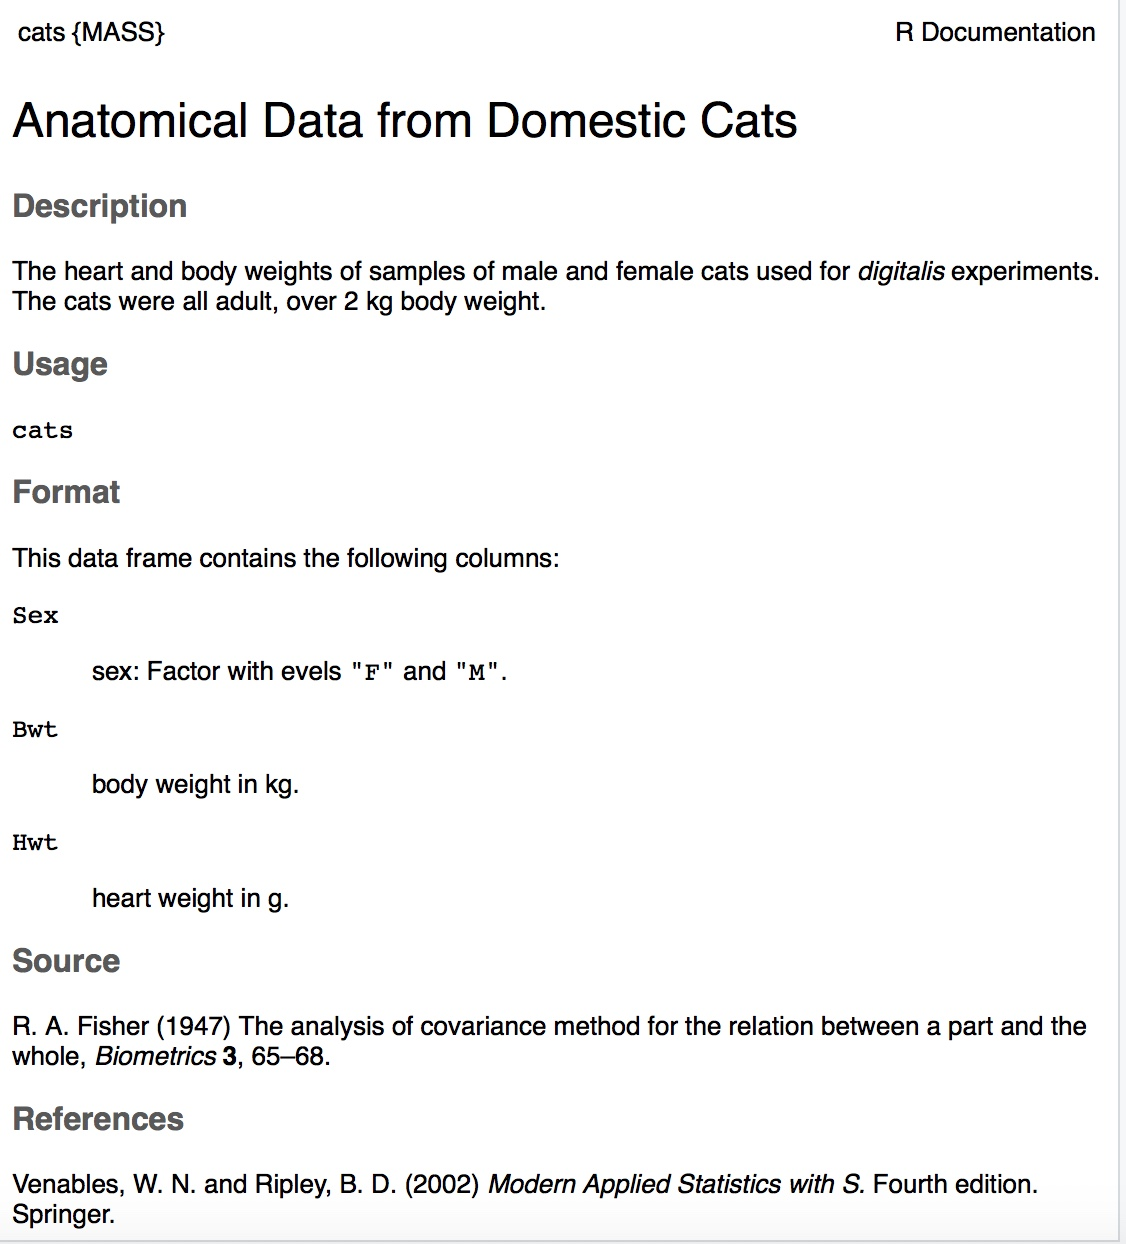
\includegraphics{code_book_cats.jpeg}

Suppose you want to know if male cats weight more than female cats. Looking at the variables, you notice that there is a variable for the sex of the cat. You can look at the weights of males and females separately. This looks like:

\begin{quote}
\textbf{Solution:}
To find the mean and median, separated by sex, use this command in R Studio:
\end{quote}

\begin{Shaded}
\begin{Highlighting}[]
\KeywordTok{df_stats}\NormalTok{(Bwt}\OperatorTok{~}\NormalTok{Sex, }\DataTypeTok{data=}\NormalTok{cats, mean, median)}
\end{Highlighting}
\end{Shaded}

\begin{verbatim}
##   Sex mean_Bwt median_Bwt
## 1   F 2.359574        2.3
## 2   M 2.900000        2.9
\end{verbatim}

\begin{quote}
Notice that the female cats' mean weigh 2.4 kg and the male cats' mean weigh 2.9 kg The median weight of female cats is 2.3 kg and for males is is 2.9 kg So it does appear that males cats weight a bit more than the female cats.
\end{quote}

There are many different summary statistics that can be found. An example is the minimum and maximum value. In this example, you will see how to find the min and max values and then filter them out of a data set to see what effect they have on the mean and median.

\hypertarget{example-affect-of-extreme-values-on-mean-and-median}{%
\subsection{Example: Affect of Extreme Values on Mean and Median**}\label{example-affect-of-extreme-values-on-mean-and-median}}

Find the minimum and maximum values of cats weights.

\begin{quote}
\textbf{Solution}
The command in R Studio for finding the minimum and maximum is very simliar to how to find the mean and median, In fact all summary statistics start with df\_stats(\textasciitilde{}variable, data=Data Frame, desired statistics). Here is the command in R Studio for the minimum and maximum of cat's body weight.
\end{quote}

\begin{Shaded}
\begin{Highlighting}[]
\KeywordTok{df_stats}\NormalTok{(}\OperatorTok{~}\NormalTok{Bwt, }\DataTypeTok{data=}\NormalTok{cats, min, max)}
\end{Highlighting}
\end{Shaded}

\begin{verbatim}
##   min_Bwt max_Bwt
## 1       2     3.9
\end{verbatim}

\begin{quote}
The minimum weigth of a cat in this data frame is 2 kg and the maximum weight of a cat is 3.9 kg.

Now create two new datasets. One data set will exclude the maximum value. You can call it anything you want, but it would make sense to call it something like nomax. The command to create the new data set is:
\end{quote}

\begin{Shaded}
\begin{Highlighting}[]
\NormalTok{nomax<-}\KeywordTok{filter}\NormalTok{(cats, Bwt}\OperatorTok{<}\FloatTok{3.9}\NormalTok{)}
\end{Highlighting}
\end{Shaded}

\begin{quote}
Then create a data set that excludes the minimmum value; call it nomin:
\end{quote}

\begin{Shaded}
\begin{Highlighting}[]
\NormalTok{nomin<-}\KeywordTok{filter}\NormalTok{(cats, Bwt}\OperatorTok{>}\DecValTok{2}\NormalTok{)}
\end{Highlighting}
\end{Shaded}

\begin{quote}
The \textless{}- is the way to indicate to R what the data set nomin is equivalent to what follows the symbol. Notice that it doesn't look like anything hapened, but new datsets were created in the background. Now you can find the mean and median of each new data set:
\end{quote}

\begin{Shaded}
\begin{Highlighting}[]
\KeywordTok{df_stats}\NormalTok{(}\OperatorTok{~}\NormalTok{Bwt, }\DataTypeTok{data=}\NormalTok{nomax, mean, median)}
\end{Highlighting}
\end{Shaded}

\begin{verbatim}
##   mean_Bwt median_Bwt
## 1 2.707042        2.7
\end{verbatim}

\begin{quote}
The mean without the maximum value is 2.70 kg, and the median is 2.7 kg.
\end{quote}

\begin{Shaded}
\begin{Highlighting}[]
\KeywordTok{df_stats}\NormalTok{(}\OperatorTok{~}\NormalTok{Bwt, }\DataTypeTok{data=}\NormalTok{nomin, mean, median)}
\end{Highlighting}
\end{Shaded}

\begin{verbatim}
##   mean_Bwt median_Bwt
## 1  2.74964        2.7
\end{verbatim}

\begin{quote}
The mean without the minimum value is 2.75 kg, and the median is 2.7 kg.
\end{quote}

From Example 3.1.1, the mean of the data set with all the values is 2.72 kg where the median is 2.7 kg. Notice that when the maximum value was excluded from the data set, the mean decreased a little but the median didn't change, and when the minimum value was excluded from the data set, the mean increased a little but the median didn't change. The mean is much higher than the median. Why is this? This is because the mean is affected by extreme values, while the median is not. We say the median is a much more resistant measure of center because it isn't affected by extreme values as much.

An outlier is a data value that is very different from the rest of the data. It can be really high or really low. Extreme values may be an outlier if the extreme value is far enough from the center. If there are extreme values in the data, the median is a better measure of the center than the mean. If there are no extreme values, the mean and the median will be similar so most people use the mean. The mean is not a resistant measure because it is affected by extreme values. The median is a resistant measure because it not affected by extreme values.

As a consumer you need to be aware that people choose the measure of center that best supports their claim. When you read an article in the newspaper and it talks about the ``average'' it usually means the mean but sometimes it refers to the median. Some articles will use the word ``median'' instead of ``average'' to be more specific. If you need to make an important decision and the information says ``average'', it would be wise to ask if the ``average'' is the mean or the median before you
decide.

As an example, suppose that a company wants to use the mean salary as the average salary for the company. This is because the high salaries of the administrators will pull the mean higher. The company can say that the employees are paid well because the average is high. However, the employees want to use the median since it discounts the extreme values of the administration and will give a lower value of the average. This will make the salaries seem lower and that a raise is in order.

Why use the mean instead of the median? The reason is because when multiple samples are taken from the same population, the sample means tend to be more consistent than other measures of the center.

To understand how the different measures of center related to skewed or symmetric distributions, see figure \#3.1.2. As you can see sometimes the mean is smaller than the median, sometimes the mean is
larger than the median, and sometimes they are the same values.

\textbf{Figure \#3.1.2: Mean, Median, Mode as Related to a Distribution}
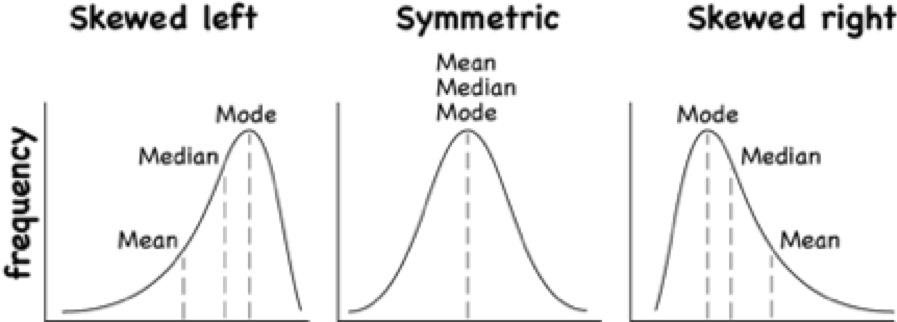
\includegraphics{centers_distribution.png}

One last type of average is a weighted average. \textbf{Weighted averages} are used quite often in different situations. Some teachers use them in calculating a student's grade in the course, or a grade on a project. Some employers use them in employee evaluations. The idea is that some activities are more
important than others. As an example, a full time teacher at a community college may be evaluated on their service to the college, their service to the community, whether their paperwork is turned in on time, and their teaching. However, teaching is much more important than whether their paperwork is turned in on time. When the evaluation is completed, more weight needs to be given to the teaching and less to the paperwork. This is a weighted average.

\begin{quote}
\textbf{Weighted Average}
\(\text{weighted average}=\frac{\sum{x*w}}{\sum{w}}\)

where \emph{w} is the weight of the data value, \emph{x}.
\end{quote}

\hypertarget{example-weighted-average}{%
\subsection{Example: Weighted Average**}\label{example-weighted-average}}

In your biology class, your final grade is based on several things: a lab score, scores on two major tests, and your score on the final exam. There are 100 points available for each score. The lab score is worth 15\% of the course, the two exams are worth 25\% of the course each, and the final exam is worth 35\% of the course. Suppose you earned scores of 95 on the labs, 83 and 76 on the two exams, and 84 on the final exam. Compute your weighted average for the course.

\begin{quote}
\textbf{Solution:}

Variable: \emph{x} = score

A weighted average can be found using technology.
The commands for finding the weighted mean using R Studio is as follows:

x\textless{}-c(type in the scores with commas in between)

w\textless{}-c(type in the weights with commas in between

weighted.mean(x,w)

The \emph{x} and \emph{w} represent the variables, \textless{}- means make the variables equivalent to what follows, the c( means combine all the values in the () as one combined variable.

For this example, the commands would be
\end{quote}

\begin{Shaded}
\begin{Highlighting}[]
\NormalTok{x<-}\KeywordTok{c}\NormalTok{(}\DecValTok{95}\NormalTok{, }\DecValTok{83}\NormalTok{, }\DecValTok{76}\NormalTok{, }\DecValTok{84}\NormalTok{)}
\NormalTok{w<-}\KeywordTok{c}\NormalTok{(.}\DecValTok{15}\NormalTok{, }\FloatTok{.25}\NormalTok{, }\FloatTok{.25}\NormalTok{, }\FloatTok{.35}\NormalTok{)}
\KeywordTok{weighted.mean}\NormalTok{(x,w)}
\end{Highlighting}
\end{Shaded}

\begin{verbatim}
## [1] 83.4
\end{verbatim}

\begin{quote}
Your weighted mean in the biology class is 83.4\%. Using the traditional grading scale, you have a B in the class.
\end{quote}

\hypertarget{example-weighted-average-1}{%
\subsection{Example: Weighted Average**}\label{example-weighted-average-1}}

The faculty evaluation process at John Jingle University rates a faculty member on the following activities: teaching, publishing, committee service, community service, and submitting paperwork in a timely manner. The process involves reviewing student evaluations, peer evaluations, and supervisor evaluation for each teacher and awarding him/her a score on a scale from 1 to 10 (with 10 being the best). The weights for each activity are 20 for teaching, 18 for publishing, 6 for committee service, 4 for community service, and 2 for paperwork.

\begin{enumerate}
\def\labelenumi{\alph{enumi})}
\tightlist
\item
  One faculty member had the following ratings: 8 for teaching, 9 for publishing, 2 for committee work, 1 for community service, and 8 for paperwork. Compute the weighted average of the evaluation.
\end{enumerate}

\begin{quote}
\textbf{Solution:}

Variable: \emph{x} = rating, \emph{w} = weight
\end{quote}

\begin{Shaded}
\begin{Highlighting}[]
\NormalTok{x<-}\KeywordTok{c}\NormalTok{(}\DecValTok{8}\NormalTok{, }\DecValTok{9}\NormalTok{, }\DecValTok{2}\NormalTok{, }\DecValTok{1}\NormalTok{, }\DecValTok{8}\NormalTok{)}
\NormalTok{w<-}\KeywordTok{c}\NormalTok{(}\DecValTok{20}\NormalTok{, }\DecValTok{18}\NormalTok{, }\DecValTok{6}\NormalTok{, }\DecValTok{4}\NormalTok{, }\DecValTok{2}\NormalTok{)}
\KeywordTok{weighted.mean}\NormalTok{(x,w)}
\end{Highlighting}
\end{Shaded}

\begin{verbatim}
## [1] 7.08
\end{verbatim}

\begin{quote}
The weighted average is 7.08.
\end{quote}

\begin{enumerate}
\def\labelenumi{\alph{enumi})}
\setcounter{enumi}{1}
\tightlist
\item
  Another faculty member had ratings of 6 for teaching, 8 for publishing, 9 for committee work, 10 for community service, and 10 for paperwork. Compute the weighted average of the evaluation.
\end{enumerate}

\begin{quote}
\textbf{Solution:}
\end{quote}

\begin{Shaded}
\begin{Highlighting}[]
\NormalTok{x<-}\KeywordTok{c}\NormalTok{(}\DecValTok{6}\NormalTok{, }\DecValTok{8}\NormalTok{, }\DecValTok{9}\NormalTok{, }\DecValTok{10}\NormalTok{, }\DecValTok{10}\NormalTok{)}
\NormalTok{w<-}\KeywordTok{c}\NormalTok{(}\DecValTok{20}\NormalTok{, }\DecValTok{18}\NormalTok{, }\DecValTok{6}\NormalTok{, }\DecValTok{4}\NormalTok{, }\DecValTok{2}\NormalTok{)}
\KeywordTok{weighted.mean}\NormalTok{(x,w)}
\end{Highlighting}
\end{Shaded}

\begin{verbatim}
## [1] 7.56
\end{verbatim}

\begin{quote}
The weighted average for this employee is 7.56.
\end{quote}

\begin{enumerate}
\def\labelenumi{\alph{enumi})}
\setcounter{enumi}{2}
\tightlist
\item
  Which faculty member had the higher average evaluation?
\end{enumerate}

\begin{quote}
\textbf{Solution:}

The second faculty member has a higher average evaluation.
\end{quote}

The last thing to mention is which average is used on which type of
data.

\begin{quote}
Mode can be found on nominal, ordinal, interval, and ratio data, since the mode is just the data value that occurs most often. You are just counting the data values.
\end{quote}

\begin{quote}
Median can be found on ordinal, interval, and ratio data, since you need to put the data in order. As long as there is order to the data you can find the median.
\end{quote}

\begin{quote}
Mean can be found on interval and ratio data, since you must have numbers to add together.
\end{quote}

\hypertarget{homework-section-3.1}{%
\subsection{Homework Section 3.1}\label{homework-section-3.1}}

** Use Technology on all problems. State the variable on all problems.**

\begin{quote}
\begin{enumerate}
\def\labelenumi{\arabic{enumi}.}
\tightlist
\item
  Cholesterol levels were collected from patients certain days after they had a heart attack and are in table \#3.1.2. Find the mean and median for cholesterol levels 2 days after the heart attack.
\end{enumerate}

table \#3.1.2
\end{quote}

\begin{Shaded}
\begin{Highlighting}[]
\NormalTok{Cholesterol<-}\KeywordTok{read.csv}\NormalTok{(}\StringTok{"https://krkozak.github.io/MAT160/cholesterol.csv"}\NormalTok{)}
\KeywordTok{head}\NormalTok{(Cholesterol)}
\end{Highlighting}
\end{Shaded}

\begin{verbatim}
##   patient day2 day4 day14
## 1       1  270  218   156
## 2       2  236  234    NA
## 3       3  210  214   242
## 4       4  142  116    NA
## 5       5  280  200    NA
## 6       6  272  276   256
\end{verbatim}

\begin{quote}
\textbf{Code book for Data Frame Cholesterol}

\textbf{Description}
Cholesterol levels were collected from patients certain days after they had a heart attack

This data frame contains the following columns:

Patient: Patient number

day2: Cholesterol level of patient 2 days after heart attack. (mg/dL)

day4: Cholesterol level of patient 4 days after heart attack. (mg/dL)

day14: Cholesterol level of patient 14 days after heart attack. (mg/dL)

\textbf{Source}
Ryan, B. F., Joiner, B. L., \& Ryan, Jr, T. A. (1985). Cholesterol levels after heart attack.Retrieved from \url{http://www.statsci.org/data/general/cholest.html}

\textbf{References}
Ryan, Joiner \& Ryan, Jr, 1985
\end{quote}

\begin{quote}
\begin{enumerate}
\def\labelenumi{\arabic{enumi}.}
\setcounter{enumi}{1}
\tightlist
\item
  The lengths (in kilometers) of rivers on the South Island of New Zealand and what body of water they flow into are listed in table \#3.1.2 (Lee, 1994). Find the mean and median length of rivers that flow into the Pacific Ocean and the mean and median length of rivers that flow into the Tasman Sea.
\end{enumerate}

** Table \#3.1.2: Lengths of Rivers (km) Flowing to Pacific Ocean**
\end{quote}

\begin{Shaded}
\begin{Highlighting}[]
\NormalTok{Length<-}\KeywordTok{read.csv}\NormalTok{(}\StringTok{"https://krkozak.github.io/MAT160/length.csv"}\NormalTok{)}
\KeywordTok{head}\NormalTok{(Length)}
\end{Highlighting}
\end{Shaded}

\begin{verbatim}
##      river length flowsto
## 1 Clarence    209 Pacific
## 2   Conway     48 Pacific
## 3    Waiau    169 Pacific
## 4  Hurunui    138 Pacific
## 5  Waipara     64 Pacific
## 6   Ashley     97 Pacific
\end{verbatim}

\begin{quote}
\textbf{Code book for data frame Length}

\textbf{Description}
Rivers in New Zealand, the lenths of river and what body of water the river flows into

This data frame contains the following columns:

River: Name of the river

length: how long the river is in kilometers

flowsto: what body of water the river flows into Pacific Ocean is Pacific and the Tasman Sea is Tasman

\textbf{Source}
Lee, A. (1994). Data analysis: An introduction based on r. Auckland. Retrieved from
\url{http://www.statsci.org/data/oz/nzrivers.html}

\textbf{References}
Lee, A. (1994). Data analysis: An introduction based on r. Auckland.
\end{quote}

\begin{quote}
\begin{enumerate}
\def\labelenumi{\arabic{enumi}.}
\setcounter{enumi}{2}
\tightlist
\item
  Print-O-Matic printing company's employees have salaries that are contained in table \#3.1.3.
\end{enumerate}

\textbf{Table \#3.1.3: Salaries of Print-O-Matic Printing Company Employees}
\end{quote}

\begin{Shaded}
\begin{Highlighting}[]
\NormalTok{Pay<-}\KeywordTok{read.csv}\NormalTok{(}\StringTok{"https://krkozak.github.io/MAT160/pay.csv"}\NormalTok{)}
\KeywordTok{head}\NormalTok{(Pay)}
\end{Highlighting}
\end{Shaded}

\begin{verbatim}
##      employee salary
## 1         CEO 272500
## 2      Driver  58456
## 3        CD74 100702
## 4        CD65  57380
## 5 Embellisher  73877
## 6      Folder  65270
\end{verbatim}

\begin{quote}
\textbf{Code book for data frame Pay}

\textbf{Description}
Salaries of Print-O-Matic printing company's employees

This data frame contains the following columns:

employee:memployees position in the company

salary: salary of that employee

\textbf{Source}
John Matic provided the data from a company he worked with. The company's name is fictitious, but the data is from an actual company.

\textbf{References}
John Matic (2013)

\begin{enumerate}
\def\labelenumi{\alph{enumi}.}
\item
  Find the mean and median.
\item
  Find the mean and median with the CEO's salary removed.
\item
  What happened to the mean and median when the CEO's salary was removed? Why?
\item
  If you were the CEO, who is answering concerns from the union that employees are underpaid, which average of the complete data set would you prefer? Why?
\item
  If you were a platen worker, who believes that the employees need a raise, which average would you prefer? Why?
\end{enumerate}
\end{quote}

\begin{quote}
\begin{enumerate}
\def\labelenumi{\arabic{enumi}.}
\setcounter{enumi}{3}
\tightlist
\item
  Print-O-Matic printing company spends specific amounts on fixed costs every month. The costs of those fixed costs are in table \#3.1.4.
  \textbf{Table \#3.1.4: Fixed Costs for Print-O-Matic Printing Company}
\end{enumerate}
\end{quote}

\begin{Shaded}
\begin{Highlighting}[]
\NormalTok{Cost<-}\KeywordTok{read.csv}\NormalTok{(}\StringTok{"https://krkozak.github.io/MAT160/cost.csv"}\NormalTok{)}
\KeywordTok{head}\NormalTok{(Cost)}
\end{Highlighting}
\end{Shaded}

\begin{verbatim}
##              charges cost
## 1       Bank charges  482
## 2           Cleaning 2208
## 3 Computer expensive 2471
## 4     Lease payments 2656
## 5            Postage 2117
## 6           Uniforms 2600
\end{verbatim}

\begin{quote}
\textbf{Code book for data frame Cost}

\textbf{Description}
fixed monthly charges for Print-0-Matic printing company

This data frame contains the following columns:

charges: Categories of monthly fixed charges

cost: fixed month costs

\textbf{Source}
John Matic provided the data from a company he worked with. The company's name is fictitious, but the data is from an actual company.

\textbf{References}
John Matic (2013)

\begin{enumerate}
\def\labelenumi{\alph{enumi}.}
\item
  Find the mean and median.
\item
  Find the mean and median with the bank charges removed.
\item
  What happened to the mean and median when the bank charges was removed? Why?
\item
  If it is your job to oversee the fixed costs, which average using the complete data set would you prefer to use when submitting a report to administration to show that costs are low? Why?
\item
  If it is your job to find places in the budget to reduce costs, which average using the complete data set would you prefer to use when submitting a report to administration to show that fixed costs need to be reduced? Why?
\end{enumerate}
\end{quote}

\begin{quote}
\begin{enumerate}
\def\labelenumi{\arabic{enumi}.}
\setcounter{enumi}{4}
\tightlist
\item
  Looking at graph \#3.1.1, state if the graph is skewed left, skewed right, or symmetric and then state which is larger, the mean or the median?
\end{enumerate}

\textbf{Graph \#3.1.1: Skewed or Symmetric Graph}
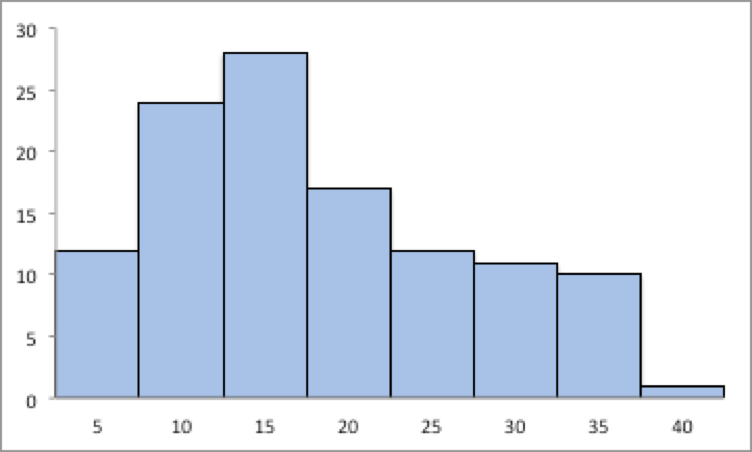
\includegraphics{graph_3_1_1.png}
\end{quote}

\begin{quote}
\begin{enumerate}
\def\labelenumi{\arabic{enumi}.}
\setcounter{enumi}{5}
\tightlist
\item
  Looking at graph \#3.1.2, state if the graph is skewed left, skewed right, or symmetric and then state which is larger, the mean or the median?
\end{enumerate}
\end{quote}

\begin{quote}
\textbf{Graph \#3.1.2: Skewed or Symmetric Graph}
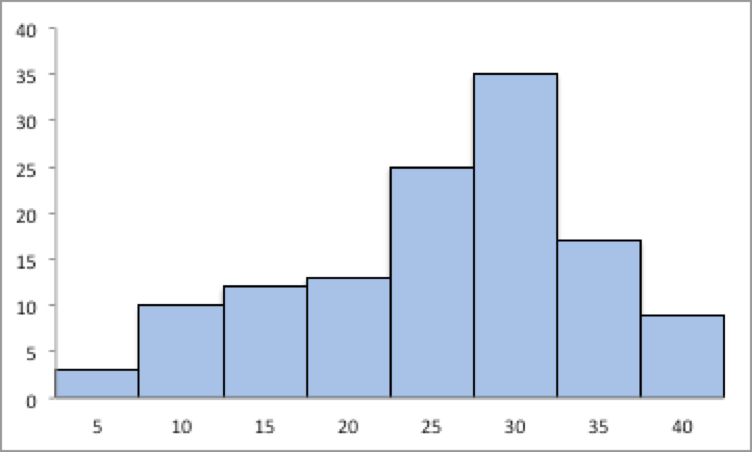
\includegraphics{graph_3_1_2.png}
\end{quote}

\begin{quote}
\begin{enumerate}
\def\labelenumi{\arabic{enumi}.}
\setcounter{enumi}{6}
\tightlist
\item
  An employee at Coconino Community College (CCC) is evaluated based on goal setting and accomplishments toward the goals, job effectiveness, competencies, and CCC core values. Suppose for a specific employee, goal 1 has a weight of 30\%, goal 2 has a weight of 20\%, job effectiveness has a weight of 25\%, competency 1 has a goal of 4\%, competency 2 has a goal has a weight of 3\%, competency 3 has a weight of 3\%, competency 4 has a weight of 3\%, competency 5 has a weight of 2\%, and core values has a weight of 10\%. Suppose the employee has scores of 3.0 for goal 1, 3.0 for goal 2, 2.0 for job effectiveness, 3.0 for competency 1, 2.0 for competency 2, 2.0 for competency 3, 3.0 for competency 4, 4.0 for competency 5, and 3.0 for core values. Find the weighted average score for this employee. If an employee has a score less than 2.5, they must have a Performance Enhancement Plan written. Does this employee need a plan?
\end{enumerate}
\end{quote}

\begin{quote}
\begin{enumerate}
\def\labelenumi{\arabic{enumi}.}
\setcounter{enumi}{7}
\tightlist
\item
  An employee at Coconino Community College (CCC) is evaluated based on goal setting and accomplishments toward goals, job effectiveness, competencies, CCC core values. Suppose for a specific employee, goal 1 has a weight of 20\%, goal 2 has a weight of 20\%, goal 3 has a weight of 10\%, job effectiveness has a weight of 25\%, competency 1 has a goal of 4\%, competency 2 has a goal has a weight of 3\%, competency 3 has a weight of 3\%, competency 4 has a weight of 5\%, and core values has a weight of 10\%. Suppose the employee has scores of 2.0 for goal 1, 2.0 for goal 2, 4.0 for goal 3, 3.0 for job effectiveness, 2.0 for competency 1, 3.0 for competency 2, 2.0 for competency 3, 3.0 for competency 4, and 4.0 for core values. Find the weighted average score for this employee. If an employee that has a score less than 2.5, they must have a Performance Enhancement Plan written. Does this employee need a plan?
\end{enumerate}
\end{quote}

\begin{quote}
\begin{enumerate}
\def\labelenumi{\arabic{enumi}.}
\setcounter{enumi}{8}
\tightlist
\item
  A statistics class has the following activities and weights for determining a grade in the course: test 1 worth 15\% of the grade, test 2 worth 15\% of the grade, test 3 worth 15\% of the grade, homework worth 10\% of the grade, semester project worth 20\% of the grade, and the final exam worth 25\% of the grade. If a student receives an 85 on test 1, a 76 on test 2, an 83 on test 3, a 74 on the homework, a 65 on the project, and a 79 on the final, what grade did the student earn in the course?
\end{enumerate}
\end{quote}

\begin{quote}
\begin{enumerate}
\def\labelenumi{\arabic{enumi}.}
\setcounter{enumi}{9}
\tightlist
\item
  A statistics class has the following activities and weights for determining a grade in the course: test 1 worth 15\% of the grade, test 2 worth 15\% of the grade, test 3 worth 15\% of the grade, homework worth 10\% of the grade, semester project worth 20\% of the grade, and the final exam worth 25\% of the grade. If a student receives a 92 on test 1, an 85 on test 2, a 95 on test 3, a 92 on the homework, a 55 on the project, and an 83 on the final, what grade did the student earn in the course?
\end{enumerate}
\end{quote}

\textbf{\\
}

\hypertarget{measures-of-spread}{%
\section{Measures of Spread}\label{measures-of-spread}}

\begin{quote}
Variability is an important idea in statistics. If you were to measure the height of everyone in your classroom, every observation gives you a different value. That means not every student has the same height. Thus there is variability in people's heights. If you were to take a sample of the income level of people in a town, every sample gives you different information. There is variability between samples too. Variability describes how the data are spread out. If the data are very close to each other, then there is low variability. If the data are very spread out, then there is high variability. How do you measure variability? It would be good to have a number that measures it. This section will describe some of the different measures of variability, also known as variation.
\end{quote}

\begin{quote}
In example \#3.1.1, the average weight of a cat was calculated to be 2.72 kg. How much does this tell you about the weight of all cats? Can you tell if most of the weights were close to 2.72 kg or were the weights really spread out? The highest weight and the lowest weight are known, but is there more that you can tell? All you know is that the center of the weights is 2.72 kg.
\end{quote}

You need more information.

\begin{quote}
The \textbf{range} of a set of data is the difference between the highest and the lowest data values (or maximum and minimum values).
\end{quote}

\hypertarget{example-range}{%
\subsection{Example: Range**}\label{example-range}}

From example \#3.1.2, the maximum is 3.9 kg and the minimum is 2 kg. So the range is \(3.9-2=1.9 kg\). But what does that tell you? You don't know if the weights are really spread out, or if they are close together.

Unfortunately, range doesn't really provide a very accurate picture of the variability. A better way to describe how the data is spread out is needed. Instead of looking at the distance the highest value is from the lowest how about looking at the distance each value is from the mean. This distance is called the \textbf{deviation}. You might want to find the average of the deviation. Though the calculation for finding the average deviation is not very straight forward, you end up with a value called the ** variance **. The symbol for the population variance is \(\sigma^2\), and it is the average squared distance from the mean. Statisticians like the variance, but many other people who work with statistics use a descriptive statistics which is the square root of the variance. This gives you the average distance from the mean. This is called the standard deviation, and is denoted with the letter \emph{s}.

\begin{quote}
The standard deviation is the average (mean) distance from a data point
to the mean. It can be thought of as how much a typical data point
differs from the mean.

The \textbf{sample variance} formula:
\(s^2=\frac{\sum\left(x-\bar{x}\right)^2}{n-1}\), where \(\bar{x}\) is the sample mean, \emph{n} is the sample size, and \(\sum{}\) means to find the sum of the data.

The \textbf{sample standard deviation} formula:
\(s=\sqrt{ \frac{\sum\left(x-\bar{x}\right)^2}{n-1}}\), the \(n-1\) on the bottom has to do with a concept called degrees of freedom. Basically, it makes the sample standard deviation a better approximation of the population standard deviation.

The \textbf{population variance} formula:
\(\sigma^2 = \frac{\sum\left(x-\mu \right)^2}{N}\), where \(\sigma\) is the Greek letter sigma and represents the population variance,
\(\mu\) is the population mean, and N is the size of the population.

The \textbf{population standard deviation} formula:
\(\sigma =\sqrt{ \frac{\sum\left(x-\mu \right)^2}{N}}\)

Both the sample variance and sample standard deviation can be found using technology. If using R Studio, you would use df\_stats(\textasciitilde{}variable, data=data frame, var, sd).
\end{quote}

The next example will demonstrate this command.

\hypertarget{example-finding-the-standard-deviation}{%
\subsection{Example: Finding the Standard Deviation**}\label{example-finding-the-standard-deviation}}

For the data frame \emph{Cats} from example \#3.2.1, find the variance and standard derivation for weight of cats. Then find the variance and standard deviation separated by sex of the cat.

\begin{quote}
\textbf{Solution:}
The variance and standard deviation for all cats is found by performing the command:
\end{quote}

\begin{Shaded}
\begin{Highlighting}[]
\KeywordTok{df_stats}\NormalTok{(}\OperatorTok{~}\NormalTok{Bwt, }\DataTypeTok{data=}\NormalTok{cats, var, sd)}
\end{Highlighting}
\end{Shaded}

\begin{verbatim}
##     var_Bwt    sd_Bwt
## 1 0.2355225 0.4853066
\end{verbatim}

\begin{quote}
The variance for all cats is 0.24 \(kg^2\) and the standard deviation is -.49 kg.

To find out the mean, variance, and standard deviation for each sex of the cats, use the command:
\end{quote}

\begin{Shaded}
\begin{Highlighting}[]
\KeywordTok{df_stats}\NormalTok{(Bwt}\OperatorTok{~}\NormalTok{Sex, }\DataTypeTok{data=}\NormalTok{cats, mean, var, sd)}
\end{Highlighting}
\end{Shaded}

\begin{verbatim}
##   Sex mean_Bwt    var_Bwt    sd_Bwt
## 1   F 2.359574 0.07506938 0.2739879
## 2   M 2.900000 0.21854167 0.4674844
\end{verbatim}

\begin{quote}
You can see that the mean weight of females cats is 2.36 kg, the variance is 0.075 \(kg^2\), and the standard deviation is 0.27 kg. For males cats, the mean is 2.9 kg, the variance is 0.22 \(kg^2\), and the standard deviation is 0.47 kg. This means that female cats weigh less than males and since the variance and standard deviations are much less for female cats than males cats, female cats' weights are more consistent than male cats.
\end{quote}

In general a ``small'' variance and standard deviation means the data is close together
(more consistent) and a ``large'' variance and standard deviation means the data is
spread out (less consistent). Sometimes you want consistent data and
sometimes you don't. As an example if you are making bolts, you want to
lengths to be very consistent so you want a small standard deviation. If
you are administering a test to see who can be a pilot, you want a large
standard deviation so you can tell who are the good pilots and who are
the not so good pilots.

What do ``small'' and ``large'' mean? To a bicyclist whose average speed is
20 mph, \emph{s} = 20 mph is huge. To an airplane whose average speed is 500
mph, \emph{s} = 20 mph is nothing. The ``size'' of the variation depends on the
size of the numbers in the problem and the mean. Another situation where
you can determine whether a standard deviation is small or large is when
you are comparing two different samples such as in example \#3.2.2. A
sample with a smaller standard deviation is more consistent than a
sample with a larger standard deviation.

\begin{quote}
Many other books and authors stress that there is a computational formula for calculating the standard deviation. However, this formula doesn't give you an idea of what standard deviation is and what you are doing. It is only good for doing the calculations quickly. It goes back to the days when standard deviations were calculated by hand, and the person needed a quick way to calculate the standard deviation. It is an archaic formula that this author is trying to eradicate. It is not necessary anymore, computers will do the calculations for you with as much meaning as this formula gives. It is suggested that you never use it. If you want to understand what the standard deviation is doing, then you should use the definition formula. If you want an answer quickly, use a computer.
\end{quote}

\textbf{Use of Standard Deviation}

One of the uses of the standard deviation is to describe how a population is distributed. This describes where much of the data is for most distributions. A general rule is that about 95\% of the data is within 2 standard deviations of the mean. This is not perfect, but is works for many distributions. There are rules like the empirical rule and Chebyshev's theorem that give you more detailed percentages, but 95\% in 2 standard deviations is a very good approximation.

\hypertarget{example-the-gneral-rule}{%
\subsection{Example: the gneral rule**}\label{example-the-gneral-rule}}

The U.S. Weather Service has provided the information in table \#3.2.1 about the total monthly/annual number of reported tornadoes in Oklahoma for the years 1950 to 2018. (US Department of Commerce \& Noaa, 2016)

\textbf{Table \#3.2.1: Monthyl/Annual Number of tornadoes in Oklahoma}

\begin{Shaded}
\begin{Highlighting}[]
\NormalTok{Tornado<-}\KeywordTok{read.csv}\NormalTok{(}\StringTok{"https://krkozak.github.io/MAT160/Tornado_OK.csv"}\NormalTok{)}
\KeywordTok{head}\NormalTok{(Tornado)}
\end{Highlighting}
\end{Shaded}

\begin{verbatim}
##   Year Jan Feb Mar Apr May Jun Jul Aug Sep Oct Nov Dec Annual
## 1 1950   0   1   1   5  12   1   0   0   2   1   0   0     23
## 2 1951   0   2   0  11  11  11   4   2   1   1   0   0     43
## 3 1952   0   0   0   7   5   5   4   1   0   0   0   0     22
## 4 1953   0   4   7   9   8  13   4   2   0   0   5   2     54
## 5 1954   0   0   7  13  19   4   4   2   3   1   0   0     53
## 6 1955   1   1   0  15  32  22   4   2   0   0   0   0     77
\end{verbatim}

\textbf{Code book for data frame Pulse}

\textbf{Description}
The U.S. Weather Service has collected data on the monthly and annual number of tornadoes in Oklahoma.

This data frame contains the following columns:

Year: Year from 1950-2018

Jan, Feb, Mar, Apr, May, Jun, Jul, Aug, Sep, Oct, Nov, Dec: Tornado numbers in each moth of the year

Annual: Total number of tornadoes for each year

\textbf{Source}
US Department of Commerce, \& Noaa. (2016, November 15). 1950 Oklahoma Tornadoes. Retrieved from \url{https://www.weather.gov/oun/tornadodata-ok-1950}

\textbf{References}
The data was supplied by The U.S. Weather Service

Find the general interval that contains about 95\% of the data.

\begin{quote}
\textbf{Solution:}

Variable: \emph{x} = number of annual tornadoes in Oklahoma

Find the mean and standard deviation:
\end{quote}

\begin{Shaded}
\begin{Highlighting}[]
\KeywordTok{df_stats}\NormalTok{(}\OperatorTok{~}\NormalTok{Annual, }\DataTypeTok{data=}\NormalTok{Tornado, mean, sd)}
\end{Highlighting}
\end{Shaded}

\begin{verbatim}
##   mean_Annual sd_Annual
## 1    56.02899  27.56061
\end{verbatim}

\begin{quote}
The mean is \(\mu=56\) tornadoes and the standard deviation is \(\sigma=27.6\) tornadoes. The interval will be \(\mu\pm2*\sigma=56\pm2*27.6=(0.8,111.2)\)

About 95\% of the years have between 0.8 or 1 and 111 tornadoes in Oklahoma.
\end{quote}

The general rule says that about 95\% of the data is within two
standard deviations of the mean. That percentage is fairly high. There
isn't much data outside two standard deviations. A rule that can be
followed is that if a data value is within two standard deviations, then
that value is a common data value. If the data value is outside two
standard deviations of the mean, either above or below, then the number
is uncommon. It could even be called unusual. An easy calculation that
you can do to figure it out is to find the difference between the data
point and the mean, and then divide that answer by the standard
deviation. As a formula this would be

\(z=\frac{x-\mu}{\sigma}\)

If you don't know the population mean, \(\mu\), and the population standard
deviation, \(\sigma\), then use the sample mean, \(\bar{x}\), and the sample standard
deviation, \emph{s}, to estimate the population parameter values. Realize that using the sample standard deviation may not actually be very accurate.

\hypertarget{example-determining-if-a-value-is-unusual}{%
\subsection{Example: Determining If a Value Is Unusual**}\label{example-determining-if-a-value-is-unusual}}

\begin{enumerate}
\def\labelenumi{\alph{enumi}.}
\tightlist
\item
  In 1974, there were 45 tornadoes in Oklahoma. Is this value unusual? Why or why not?
\end{enumerate}

\begin{quote}
\textbf{Solution:}

Variable: \emph{x} = number of tornadoes in Oklahoma

To answer this question, first find how many standard deviations 45 is from the mean. From example \#3.2.3, we know \(\mu=56\) and \(\sigma=27.6\). For \emph{x}=45, \(z=\frac{45-56}{27.6}=-0.399\)

Since this value is between -2 and 2, then it is not unusual to have 45 tornadoes in a year in Oklahoma. The z vlaue is negative, so that means that 45 is less than the mean number of tornadoes.
\end{quote}

\begin{enumerate}
\def\labelenumi{\alph{enumi}.}
\setcounter{enumi}{1}
\tightlist
\item
  In 1999, there were 145 tornadoes in the Oklahoma. Is this value unusual? Why or why not?
\end{enumerate}

\begin{quote}
\textbf{Solution:}

Variable: \emph{x} = number of tornadoes in Oklahoma

For this question the \emph{x} = 145, \(z=\frac{145-56}{27.6}=3.22\)

Since this value is more than 2, then it is unusual to have only 145 tornadoes in a year in Oklahoma.
\end{quote}

\hypertarget{homework-section-3.2}{%
\subsection{Homework Section 3.2}\label{homework-section-3.2}}

\textbf{Use Technology on all problems. State the variable on all problems.}

\begin{quote}
\begin{enumerate}
\def\labelenumi{\arabic{enumi}.}
\tightlist
\item
  Cholesterol levels were collected from patients certain days after they had a heart attack and are in table \#3.2.2. Find the mean, median, range, variance, and standard deviation for cholesterol levels 2 days after the heart attack.
\end{enumerate}

\textbf{table \#3.3.2: Cholesterol Levels of Patients After Heart Attack}
\end{quote}

\begin{Shaded}
\begin{Highlighting}[]
\NormalTok{Cholesterol<-}\KeywordTok{read.csv}\NormalTok{(}\StringTok{"https://krkozak.github.io/MAT160/cholesterol.csv"}\NormalTok{)}
\KeywordTok{head}\NormalTok{(Cholesterol)}
\end{Highlighting}
\end{Shaded}

\begin{verbatim}
##   patient day2 day4 day14
## 1       1  270  218   156
## 2       2  236  234    NA
## 3       3  210  214   242
## 4       4  142  116    NA
## 5       5  280  200    NA
## 6       6  272  276   256
\end{verbatim}

\begin{quote}
\textbf{Code book for Data Frame Cholesterol} See problem 3.1.1 in Section 3.1 homework.
\end{quote}

\begin{quote}
\begin{enumerate}
\def\labelenumi{\arabic{enumi}.}
\setcounter{enumi}{1}
\tightlist
\item
  The lengths (in kilometers) of rivers on the South Island of New Zealand and what body of water they flow into are listed in table \#3.1.2 (Lee, 1994). Find the mean, median, range, variance, and standard deviation of the length of rivers that flow into the Pacific Ocean and the mean, median, range, variance, and standard deviation of the length of rivers that flow into the Tasman Sea. Compare and contrast the length of rivers that flow to the Pacific Ocean versus the ones that flow into the Tasman Sea using both measures of spread and measures of variability.
\end{enumerate}

\textbf{Table \#3.3.3: Lengths of Rivers (km) Flowing to Pacific Ocean}
\end{quote}

\begin{Shaded}
\begin{Highlighting}[]
\NormalTok{Length<-}\KeywordTok{read.csv}\NormalTok{(}\StringTok{"https://krkozak.github.io/MAT160/length.csv"}\NormalTok{)}
\KeywordTok{head}\NormalTok{(Length)}
\end{Highlighting}
\end{Shaded}

\begin{verbatim}
##      river length flowsto
## 1 Clarence    209 Pacific
## 2   Conway     48 Pacific
## 3    Waiau    169 Pacific
## 4  Hurunui    138 Pacific
## 5  Waipara     64 Pacific
## 6   Ashley     97 Pacific
\end{verbatim}

\begin{quote}
\textbf{Code book for data frame Length} See problem 3.1.2 in Section 3.1 homework.
\end{quote}

\begin{quote}
\begin{enumerate}
\def\labelenumi{\arabic{enumi}.}
\setcounter{enumi}{2}
\tightlist
\item
  Print-O-Matic printing company's employees have salaries that are contained in table \#3.2.4. Find the mean, median, range, variance, and standard deviation for the salaries of all employees.
\end{enumerate}

\textbf{Table \#3.2.4: Salaries of Print-O-Matic Printing Company Employees}
\end{quote}

\begin{Shaded}
\begin{Highlighting}[]
\NormalTok{Pay<-}\KeywordTok{read.csv}\NormalTok{(}\StringTok{"https://krkozak.github.io/MAT160/pay.csv"}\NormalTok{)}
\KeywordTok{head}\NormalTok{(Pay)}
\end{Highlighting}
\end{Shaded}

\begin{verbatim}
##      employee salary
## 1         CEO 272500
## 2      Driver  58456
## 3        CD74 100702
## 4        CD65  57380
## 5 Embellisher  73877
## 6      Folder  65270
\end{verbatim}

\begin{quote}
\textbf{Code book for data frame Pay} See problem 3.1.3 in Section 3.1 homework.
\end{quote}

\begin{quote}
\begin{enumerate}
\def\labelenumi{\arabic{enumi}.}
\setcounter{enumi}{3}
\tightlist
\item
  Print-O-Matic printing company spends specific amounts on fixed costs every month. The costs of those fixed costs are in table \#3.2.5. Find the mean, median, range, variance, and standard deviation for the fixed costs.
\end{enumerate}

\textbf{Table \#3.2.5: Fixed Costs for the Print-O-Matic Printing Company}
\end{quote}

\begin{Shaded}
\begin{Highlighting}[]
\NormalTok{Cost<-}\KeywordTok{read.csv}\NormalTok{(}\StringTok{"https://krkozak.github.io/MAT160/cost.csv"}\NormalTok{)}
\KeywordTok{head}\NormalTok{(Cost)}
\end{Highlighting}
\end{Shaded}

\begin{verbatim}
##              charges cost
## 1       Bank charges  482
## 2           Cleaning 2208
## 3 Computer expensive 2471
## 4     Lease payments 2656
## 5            Postage 2117
## 6           Uniforms 2600
\end{verbatim}

\begin{quote}
\textbf{Code book for Data frame Cost} See problem 3.1.4 in Section 3.1 homework.
\end{quote}

\begin{quote}
\begin{enumerate}
\def\labelenumi{\arabic{enumi}.}
\setcounter{enumi}{4}
\tightlist
\item
  The data frame Pulse (Table 3.2.6) contains various variables about a person including their pulse rates before the subject exercised and after after the subject ran in place for one minute.
\end{enumerate}

\textbf{Table \#3.2.6: Pulse Rates of people Before and After Exercise}
\end{quote}

\begin{Shaded}
\begin{Highlighting}[]
\NormalTok{Pulse<-}\KeywordTok{read.csv}\NormalTok{(}\StringTok{"https://krkozak.github.io/MAT160/pulse.csv"}\NormalTok{)}
\KeywordTok{head}\NormalTok{(Pulse)}
\end{Highlighting}
\end{Shaded}

\begin{verbatim}
##   height weight age gender smokes alcohol exercise ran pulse_before
## 1    170     68  22   male    yes     yes moderate sat           70
## 2    182     75  26   male    yes     yes moderate sat           80
## 3    180     85  19   male    yes     yes moderate ran           68
## 4    182     85  20   male    yes     yes      low sat           70
## 5    167     70  22   male    yes     yes      low sat           92
## 6    178     86  21   male    yes     yes      low sat           76
##   pulse_after year
## 1          71   93
## 2          76   93
## 3         125   95
## 4          68   95
## 5          84   96
## 6          80   98
\end{verbatim}

\begin{quote}
\textbf{Code book for data frame Pulse}

\textbf{Description}
Students in an introductory statistics class (MS212 taught by Professor John Eccleston and Dr Richard Wilson at The University of Queensland) participated in a simple experiment. The students took their own pulse rate. They were then asked to flip a coin. If the coin came up heads, they were to run in place for one minute. Otherwise they sat for one minute. Then everyone took their pulse again. The pulse rates and other physiological and lifestyle data are given in the data.

Five class groups between 1993 and 1998 participated in the experiment. The lecturer, Richard Wilson, was concerned that some students would choose the less strenuous option of sitting rather than running even if their coin came up heads, In the years 1995-1998 a different method of random assignment was used. In these years, data forms were handed out to the class before the experiment. The forms were pre-assigned to either running or non-running and there were an equal number of each. In 1995 and 1998 not all of the forms were returned so the numbers running and sitting was still not entirely controlled.

This data frame contains the following columns:

height: height of subject in cm

weight: weight of subject in kg

age: age of subject in years

gender: sex of subject, male, female

Smokes: whether a subject regularly smokes, yes means does smoke, no means does not smoke

alcohol: whether a subject regularly drinks alcohol, yes means the person does, no means the person does not

exercise: whether a subject exercises, low, moderate, high

ran: whether a subject ran one minute between pulse measurements (ran) or sat between pulse measurement (sat)

pulse\_before: the pulse rate before a subject either ran or sat (bpm)

pulse\_after: the pulse rate after a subject either ran or sat (bpm)

year: what year the data was collected (93-98)

\textbf{Source}
Pulse rates before and after exercise. (2013, September 25). Retrieved from
\url{http://www.statsci.org/data/oz/ms212.html}

\textbf{References}
The data was supplied by Dr Richard J. Wilson, Department of Mathematics, University of Queensland.

Create a data frame that contains only males, who drink alcohol, but do not smoke. Then compare the pulse before and the pulse after using the mean and standard deviation. Discuss whether pulse before or pulse after has a higher mean and larger spread. To create a new data frame with just males, who drink alcohol, but do not smoke, use the following command, where the new name is Males:
\end{quote}

\begin{Shaded}
\begin{Highlighting}[]
\NormalTok{Males<-}
\NormalTok{Pulse}\OperatorTok
\StringTok{  }\KeywordTok{filter}\NormalTok{(gender}\OperatorTok{==}\StringTok{"male"}\NormalTok{, smokes }\OperatorTok{==}\StringTok{ "no"}\NormalTok{, alcohol }\OperatorTok{==}\StringTok{ "yes"}\NormalTok{)}
\end{Highlighting}
\end{Shaded}

\begin{quote}
\begin{enumerate}
\def\labelenumi{\arabic{enumi}.}
\setcounter{enumi}{5}
\tightlist
\item
  The data frame Pulse (Table 3.2.6) contains various variables about a person including their pulse rates before the subject exercised and after after the subject ran in place for one minute. Create a data frame that contains females, who do not smoke but do drink alcohol. Compare the pulse rate before and after exercise using the mean and standard deviation. Discuss whether pulse before or pulse after has a higher mean and larger spread.
\end{enumerate}
\end{quote}

\begin{quote}
\begin{enumerate}
\def\labelenumi{\arabic{enumi}.}
\setcounter{enumi}{6}
\tightlist
\item
  To determine if Reiki is an effective method for treating pain, a pilot study was carried out where a certified second-degree Reiki therapist provided treatment on volunteers. Pain was measured using a visual analogue scale (VAS) and a likert scale immediately before and after the Reiki treatment (Olson \& Hanson, 1997) and the data is in table \#3.2.7.
\end{enumerate}

\textbf{Table \#3.2.7: Pain Measurements Before and After Reiki Treatment}
\end{quote}

\begin{Shaded}
\begin{Highlighting}[]
\NormalTok{Reiki<-}\StringTok{ }\KeywordTok{read.csv}\NormalTok{(}\StringTok{"https://krkozak.github.io/MAT160/reki.csv"}\NormalTok{)}
\KeywordTok{head}\NormalTok{(Reiki)}
\end{Highlighting}
\end{Shaded}

\begin{verbatim}
##   vas.before vas.after likert_before likert_after
## 1          6         3             2            1
## 2          2         1             2            1
## 3          2         0             3            0
## 4          9         1             3            1
## 5          3         0             2            0
## 6          3         2             2            2
\end{verbatim}

\begin{quote}
\textbf{Code book for data frame Reiki}

\textbf{Description}
The purpose of this study was to explore the usefulness of Reiki as an adjuvant to opioid therapy in the management of pain. Since no studies in this area could be found, a pilot study was carried out involving 20 volunteers experiencing pain at 55 sites for a variety of reasons, including cancer. All Reiki treatments were provided by a certified second-degree Reiki therapist. Pain was measured using both a visual analogue scale (VAS) and a Likert scale immediately before and after the Reiki treatment. Both instruments showed a highly significant (p \textless{} 0.0001) reduction in pain following the Reiki treatment.

This data frame contains the following columns:

vas.before: pain measured using a visual analogue scale (VAS) before Reiki treatment

vas.after: pain measured using a visual analogue scale (VAS) after Reiki treatment

likert\_before: pain measured using a likert before Reiki treatment

likert\_after: pain measured using a likert after Reiki treatment

\textbf{Source}
Olson, K., \& Hanson, J. (1997). Using reiki to manage pain: a preliminary report. Cancer Prev Control, 1(2), 108-13. Retrieved from \url{http://www.ncbi.nlm.nih.gov/pubmed/9765732}

\textbf{References}
Using Reiki to manage pain: a preliminary report. Olson K1, Hanson J., Cancer Prev Control 1997, Jun; 1(2): 108-13.

Since the data was collected both and before and after the treatment for all of the units of observations, you want to look at the effect size of the treatment. You want to find the difference between before and after for the pain scale. First you must create a new data frame that adds a column for the difference in before and after. This data is known as paired data. To create the new column in a new data frame called Newreiki use the following commands
\end{quote}

\begin{Shaded}
\begin{Highlighting}[]
\NormalTok{Newreiki<-Reiki}\OperatorTok
\StringTok{  }\KeywordTok{mutate}\NormalTok{(}\DataTypeTok{vas.diff=}\NormalTok{vas.before}\OperatorTok{-}\NormalTok{vas.after)}
\KeywordTok{head}\NormalTok{(Newreiki)}
\end{Highlighting}
\end{Shaded}

\begin{verbatim}
##   vas.before vas.after likert_before likert_after vas.diff
## 1          6         3             2            1        3
## 2          2         1             2            1        1
## 3          2         0             3            0        2
## 4          9         1             3            1        8
## 5          3         0             2            0        3
## 6          3         2             2            2        1
\end{verbatim}

\begin{quote}
Now find the mean and standard deviation of the vas.diff variable in Newreiki. Perform similar commands to create the likert.diff variable. Then find the mean and standard deviation for likert.diff, and compare and contrast the vas and likert methods for describing pain.
\end{quote}

\begin{quote}
8.Yearly rainfall amounts (in millimeters) in Sydney, Australia, are in table \#3.2.8
(``Annual maximums of,'' 2013).
a. Calculate the mean and standard deviation.
b. Suppose Sydney, Australia received 300 mm of rainfall in a year. Would this be unusual?

** Table \#3.2.8: Yewarly rainfall amounts in Sydney, Australia**
\end{quote}

\begin{Shaded}
\begin{Highlighting}[]
\NormalTok{Rainfall<-}\KeywordTok{read.csv}\NormalTok{(}\StringTok{"https://krkozak.github.io/MAT160/rainfall.csv"}\NormalTok{)}
\KeywordTok{head}\NormalTok{(Rainfall)}
\end{Highlighting}
\end{Shaded}

\begin{verbatim}
##   amount
## 1  146.8
## 2  383.0
## 3   90.9
## 4  178.1
## 5  267.5
## 6   95.5
\end{verbatim}

\begin{quote}
\textbf{Code book for data frame Rainfall}

\textbf{Description}
Daily rainfall (in millimetres) was recorded over a 47-year period in Turramurra, Sydney, Australia. For each year, the wettest day was identified (that having the greatest rainfall). The data show the rainfall recorded for the 47 annual maxima.

This data frame contains the following columns:

amount: daily rainfall (mm)

\textbf{Source}
Annual maximums of daily rainfall in Sydney. (2013, September 25). Retrieved from
\url{http://www.statsci.org/data/oz/sydrain.html}

\textbf{References}
Rayner J.C.W. and Best D.J. (1989) Smooth tests of goodness of fit. Oxford: Oxford University Press.
Hand D.J., Daly F., Lunn A.D., McConway K.J., Ostrowski E. (1994). A Handbook of Small Data Sets. London: Chapman \& Hall. Data set 157.
Thanks to Jim Irish of the University of Technology, Sydney, for assistance in identifying the correct units for this data.
\end{quote}

\textbf{\\
}

\hypertarget{ranking}{%
\section{Ranking}\label{ranking}}

Along with the center and the variability, another useful numerical
measure is the ranking of a number. A \textbf{percentile} is a measure of
ranking. It represents a location measurement of a data value to the
rest of the values. Many standardized tests give the results as a
percentile. Doctors also use percentiles to track a child's growth.

The \textbf{\emph{k}th percentile} is the data value that has k\% of the data at or
below that value.

\hypertarget{example-interpreting-percentile}{%
\subsection{Example: Interpreting Percentile**}\label{example-interpreting-percentile}}

\begin{enumerate}
\def\labelenumi{\alph{enumi}.}
\tightlist
\item
  What does a score of the 90\textsuperscript{th} percentile mean?
\end{enumerate}

\begin{quote}
\textbf{Solution:}

This means that 90\% of the scores were at or below this score. (A person did the same as or better than 90\% of the test takers.)

\begin{enumerate}
\def\labelenumi{\alph{enumi}.}
\setcounter{enumi}{1}
\tightlist
\item
  What does a score of the 70\textsuperscript{th} percentile mean?
\end{enumerate}
\end{quote}

\begin{quote}
\textbf{Solution:}

This means that 70\% of the scores were at or below this score.
\end{quote}

\hypertarget{example-percentile-versus-score}{%
\subsection{Example: Percentile Versus Score**}\label{example-percentile-versus-score}}

If the test was out of 100 points and you scored at the 80\textsuperscript{th} percentile, what was your score on the test?

\begin{quote}
\textbf{Solution:}

You don't know! All you know is that you scored the same as or better than 80\% of the people who took the test. If all the scores were really low, you could have still failed the test. On the other hand, if many of the scores were high you could have gotten a 95\% or more.
\end{quote}

There are special percentiles called \textbf{quartiles}. Quartiles are numbers that divide the data into fourths. One fourth (or a quarter) of the data falls between consecutive quartiles.

\textbf{To find the quartiles:}

The command in R Studio is df\_stats(\textasciitilde{}variable, data=data frame, summary)

If you record the quartiles together with the maximum and minimum you
have five numbers. This is known as the five-number summary. The
five-number summary consists of the minimum, the first quartile (\emph{Q1}),
the median, the third quartile (\emph{Q3}), and the maximum (in that order).

The interquartile range, \emph{IQR}, is the difference between the first and third quartiles, \emph{Q1} and \emph{Q3}. Half of the data (50\%) falls in the interquartile range. If the \emph{IQR} is ``large'' the data is spread out and if the \emph{IQR} is ``small'' the data is closer together.

Interquartile Range (\emph{IQR})

\textbf{Determining probable outliers from IQR: }fences**

A value that is less than (this value is often referred to as a \textbf{low} \textbf{fence}) is considered an outlier.

Similarly, a value that is more than (the \textbf{high} \textbf{fence}) is considered an outlier.

A boxplot (or box-and-whisker plot) is a graphical display of the five-number summary. It can be drawn vertically or horizontally. The basic format is a box from \emph{Q1} to \emph{Q3}, a vertical line across the box for the median and horizontal lines as whiskers extending out each end to the minimum and maximum. The minimum and maximum can be represented with dots. Don't forget to label the tick marks on the number line and give the graph a title.

An alternate form of a Boxplot, known as a modified box plot, only extends the left line to the smallest value greater than the \emph{low fence}, and extends the left line to the largest value less than
the \emph{high fence}, and displays markers (dots, circles or asterisks) for each outlier.

If the data are \emph{symmetrical}, then the box plot will be visibly symmetrical. If the data distribution has a left skew or a right skew, the line on that side of the box plot will be visibly long. If the plot is symmetrical, and the four quartiles are all about the same length, then the data are likely a near \emph{uniform} distribution. If a box plot is symmetrical, and both outside lines are noticeably longer than the Q1 to median and median to Q3 distance, the distribution is then probably
\emph{bell-shaped.}

\hypertarget{example-five-number-summary-and-boxplot}{%
\subsection{Example: Five-number Summary and Boxplot}\label{example-five-number-summary-and-boxplot}}

Find the five-number summary, the interquartile range (\emph{IQR}), and draw a box-and-whiskers plot for the weight of cats.

\begin{Shaded}
\begin{Highlighting}[]
\KeywordTok{head}\NormalTok{(cats)}
\end{Highlighting}
\end{Shaded}

\begin{verbatim}
##   Sex Bwt Hwt
## 1   F 2.0 7.0
## 2   F 2.0 7.4
## 3   F 2.0 9.5
## 4   F 2.1 7.2
## 5   F 2.1 7.3
## 6   F 2.1 7.6
\end{verbatim}

\begin{quote}
\textbf{Solution:}

Variable: \emph{x} = weight of cats
To compute the five number summary on R Studio, use the command:
\end{quote}

\begin{Shaded}
\begin{Highlighting}[]
\KeywordTok{df_stats}\NormalTok{(}\OperatorTok{~}\NormalTok{Bwt, }\DataTypeTok{data=}\NormalTok{cats, summary)}
\end{Highlighting}
\end{Shaded}

\begin{verbatim}
##   Min. 1st Qu. Median     Mean 3rd Qu. Max.
## 1    2     2.3    2.7 2.723611   3.025  3.9
\end{verbatim}

\begin{quote}
Minimum: 2 kg
\emph{Q1}: 2.3 kg
Median: 2.7 kg
\emph{Q3}: 3.025 kg
Maximum: 3.9 kg

To find the interquartile range, \emph{IQR}, find \(Q3-Q1\), so \(IQR=3.025-2.3=0.725 kg\)

To create a boxplot use the command gf\_boxplot(\textasciitilde{}variable, data=data frame). This is a modified boxplot which shows the outliers in the data.

\textbf{Graph \#3.3.1: Box Plot of Weights of Cats}
\end{quote}

\begin{Shaded}
\begin{Highlighting}[]
\KeywordTok{gf_boxplot}\NormalTok{(}\OperatorTok{~}\NormalTok{Bwt, }\DataTypeTok{data=}\NormalTok{cats, }\DataTypeTok{title=}\StringTok{"Weight of Cats"}\NormalTok{)}
\end{Highlighting}
\end{Shaded}

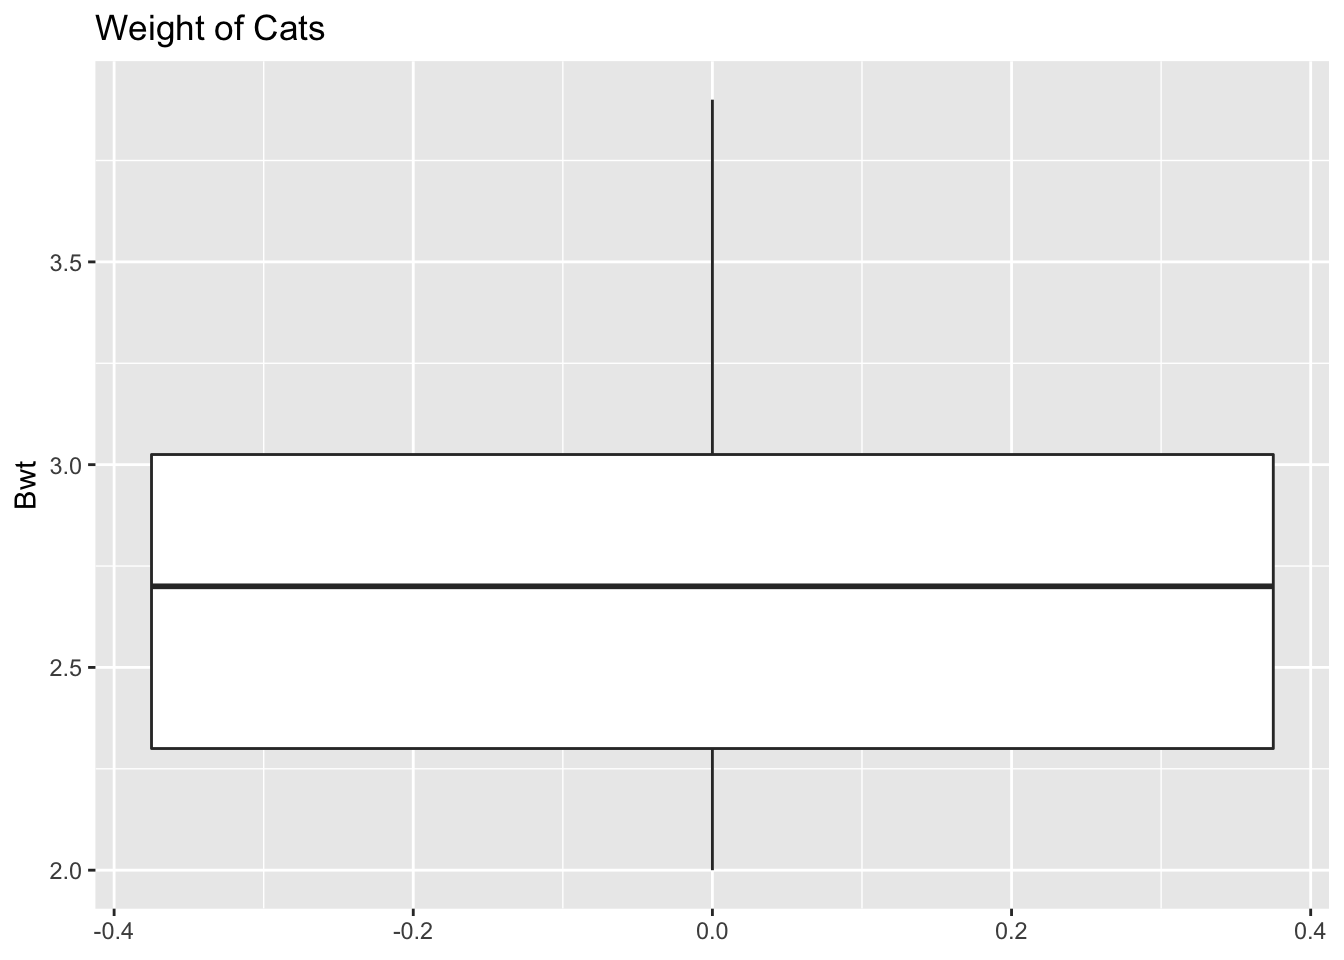
\includegraphics{Statistics_using_technology_files/figure-latex/unnamed-chunk-34-1.pdf}
\textgreater{} There are no outliers since there are no dots outside of the fences.

\hypertarget{example-separating-based-on-a-factor}{%
\subsection{Example: Separating based on a factor**}\label{example-separating-based-on-a-factor}}

Find the five-number summary of the weights of cats separated by the sex of the cat. Then create a box plot of the weights of cats for each sex of the cat.

\begin{quote}
\textbf{Solution:}

Variable: \emph{x\_1} = weight of female cat

Variable: \emph{x\_2} = weight of male cat

To find the five-number summary seperated based on genderm use the following command:
\end{quote}

\begin{Shaded}
\begin{Highlighting}[]
\KeywordTok{df_stats}\NormalTok{(}\OperatorTok{~}\NormalTok{Bwt}\OperatorTok{|}\NormalTok{Sex, }\DataTypeTok{data=}\NormalTok{cats, summary)}
\end{Highlighting}
\end{Shaded}

\begin{verbatim}
##   Sex Min. 1st Qu. Median     Mean 3rd Qu. Max.
## 1   F    2    2.15    2.3 2.359574     2.5  3.0
## 2   M    2    2.50    2.9 2.900000     3.2  3.9
\end{verbatim}

\begin{quote}
The five-number summary for female cats is (in kg)

Minimum: 2
Q1: 2.15
Median: 2.3
Q3: 2.5
Maximum: 3.0

The five-number summary for male cats is (in kg)

Minimum: 2
Q1: 2.50
Median: 2.9
Q3: 3.2
Maximum: 3.9

\textbf{Graph \#3.3.2: Box Plot of Cats Weights Separated by Sex}
\end{quote}

\begin{Shaded}
\begin{Highlighting}[]
\KeywordTok{gf_boxplot}\NormalTok{(}\OperatorTok{~}\NormalTok{Bwt}\OperatorTok{|}\NormalTok{Sex, }\DataTypeTok{data=}\NormalTok{cats, }\DataTypeTok{title=}\StringTok{"Weights of Cats"}\NormalTok{)}
\end{Highlighting}
\end{Shaded}

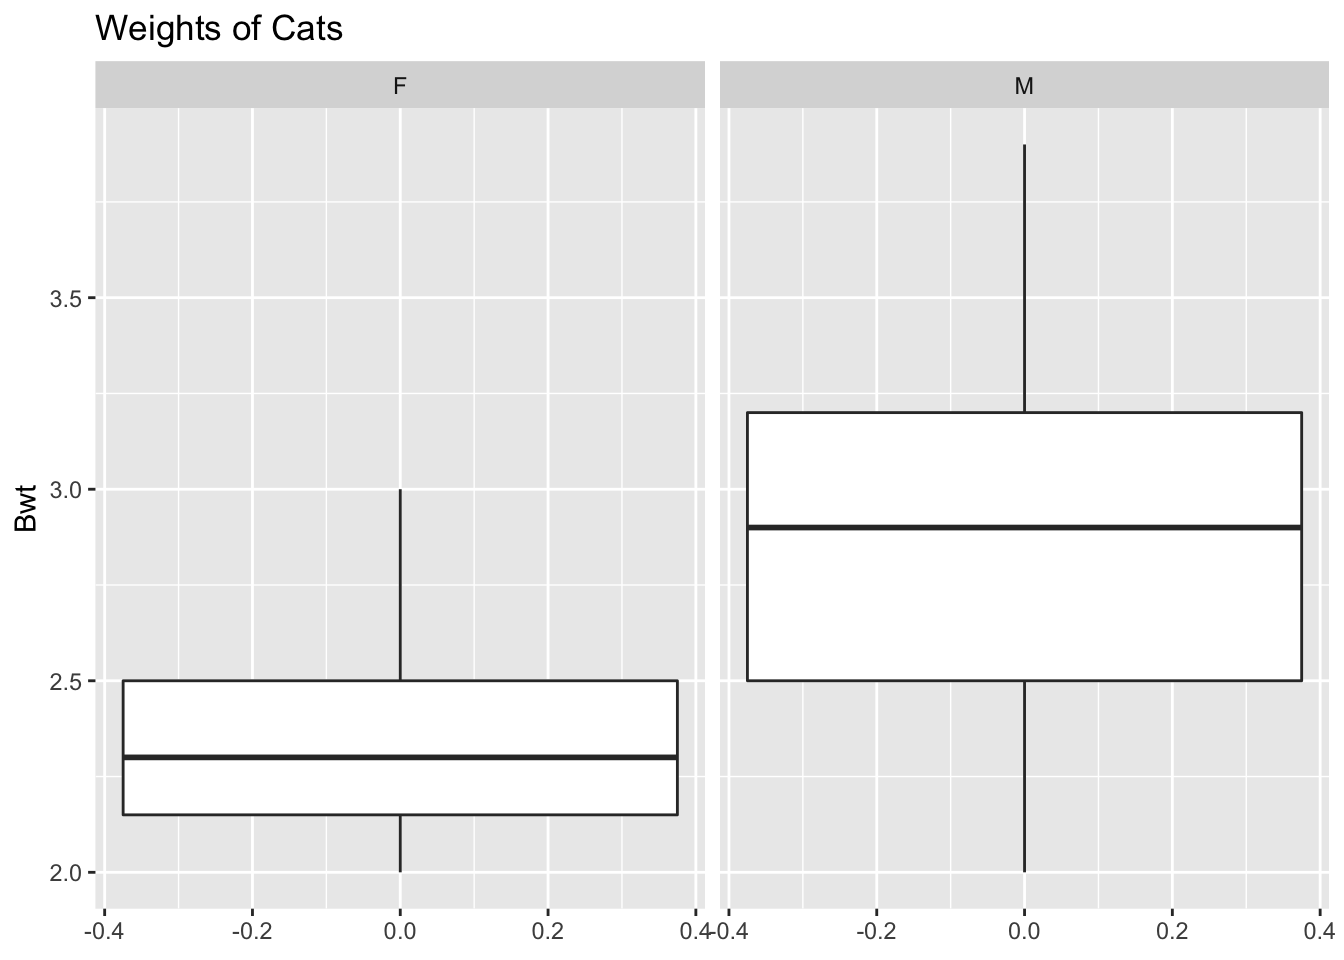
\includegraphics{Statistics_using_technology_files/figure-latex/unnamed-chunk-36-1.pdf}
\textgreater{}
\textgreater{} Notice that the weights of female cats has a median less than male cats, and in fact it can be seen that the Q1 to Q3 of the female cats is less than the Q1 to Q3 of the male cats.

\hypertarget{example-putting-it-all-together}{%
\subsection{Example: Putting it all together**}\label{example-putting-it-all-together}}

The time (in 1/50 seconds) between successive pulses along a nerve fiber (``Time
between nerve,'' 2013) are given in table \#3.3.1.

\textbf{Table \#3.3.1: Successive pulses along a nerve fiber}

\begin{Shaded}
\begin{Highlighting}[]
\NormalTok{Nerve<-}\KeywordTok{read.csv}\NormalTok{(}\StringTok{"https://krkozak.github.io/MAT160/Nerve_pulse.csv"}\NormalTok{)}
\KeywordTok{head}\NormalTok{(Nerve)}
\end{Highlighting}
\end{Shaded}

\begin{verbatim}
##   time
## 1 10.5
## 2  1.5
## 3  2.5
## 4  5.5
## 5 29.5
## 6  3.0
\end{verbatim}

\textbf{Code book for data frame Nerve}

\textbf{Description}
The data gives the time between 800 successive pulses along a nerve fiber. There are 799 observations rounded to the nearest half in units of 1/50 second.

This data frame contains the following columns:

time: time between successive Pulses along a nerve fiber, 1/50 second.

\textbf{Source}
\emph{Time between nerve pulses}. (2019, July 3). Retrieved from
\url{http://www.statsci.org/data/general/nerve.html}

\textbf{References}
Fatt, P., and Katz, B. (1952). Spontaneous subthreshold activity at motor nerve endings. Journal of Physiology 117, 109-128.

Cox, D. R., and Lewis, P. A. W. (1966). The Statistical Analysis of Series of Events. Methuen, London.

Jorgensen, B. (1982). The Generalized Inverse-Gaussian Distribution. Springer-Verlag.

\begin{quote}
\textbf{Solution:}

First, it might be useful to look at a visualization of the data, so create a density plot

\textbf{Graph \#3.3.2: Density Plot of Health Expenditure}
\end{quote}

\begin{Shaded}
\begin{Highlighting}[]
\KeywordTok{gf_density}\NormalTok{(}\OperatorTok{~}\NormalTok{time, }\DataTypeTok{data=}\NormalTok{Nerve)}
\end{Highlighting}
\end{Shaded}

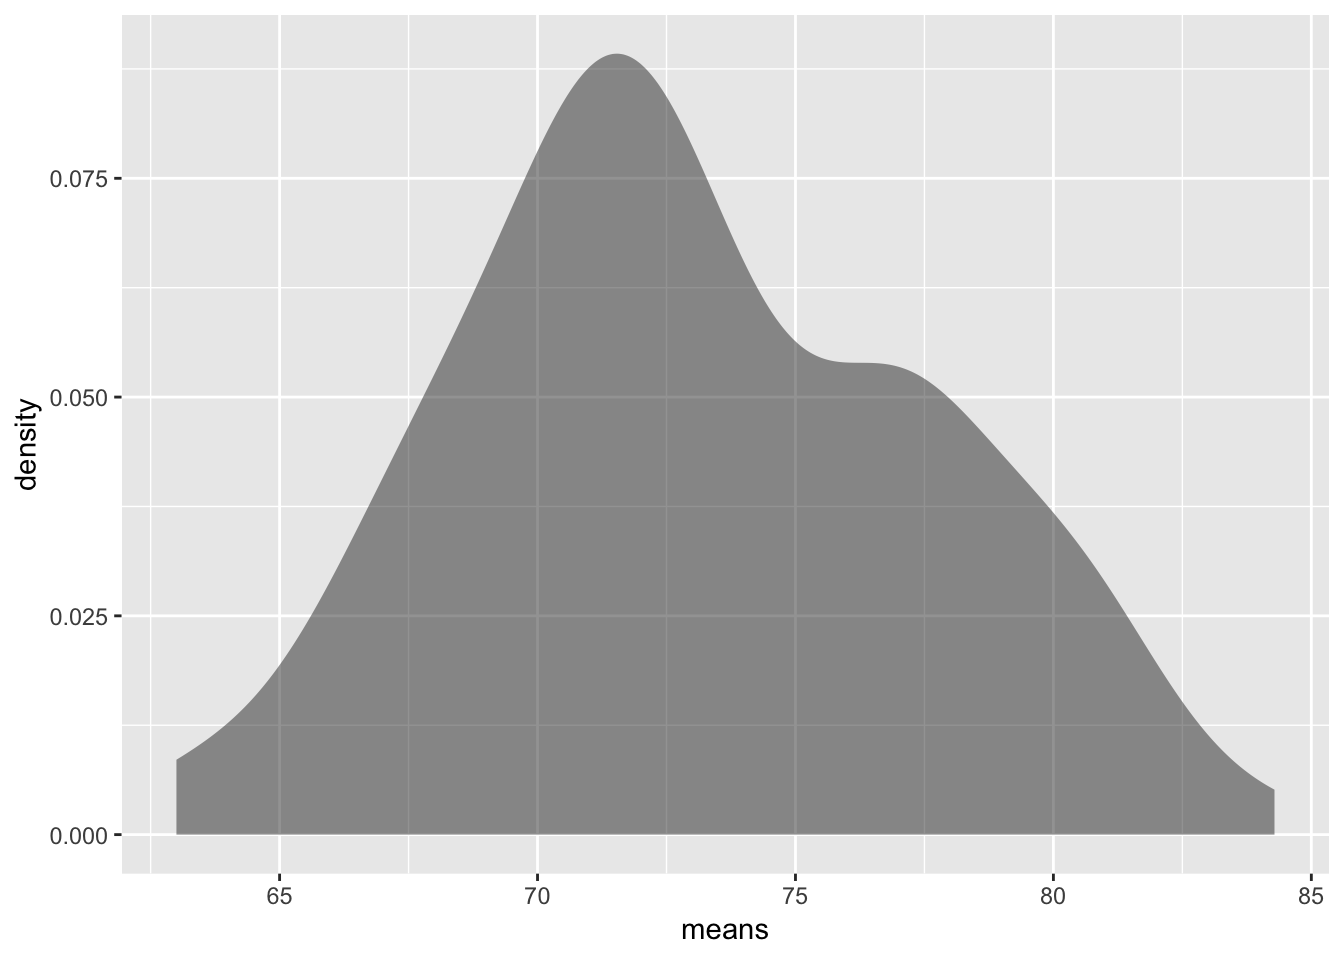
\includegraphics{Statistics_using_technology_files/figure-latex/unnamed-chunk-38-1.pdf}
\textgreater{}
\textgreater{} From the graph, the data appears to be skewed right. Most of the time between successive nerve pusles appear to be around 5 or 10 1/50 second, but there are some times that are 60 1/50 second.

\begin{Shaded}
\begin{Highlighting}[]
\KeywordTok{df_stats}\NormalTok{(}\OperatorTok{~}\NormalTok{time, }\DataTypeTok{data=}\NormalTok{Nerve, mean, median, sd, summary)}
\end{Highlighting}
\end{Shaded}

\begin{verbatim}
##   mean_time median_time  sd_time Min. 1st Qu. Median     Mean 3rd Qu. Max.
## 1  10.95119         7.5 10.45956  0.5     3.5    7.5 10.95119      15   69
\end{verbatim}

\begin{quote}
Numerical descriptions might also be useful. Using technology, the mean is 11 1/50 second,the median is 7.5 1/50 second, the standard deviation is 10.5 1/50 second, and the five-number summary is minimum = 3.5, Q1 = 3.5, median = 7.5, Q3 = 15, and maximum = 69 1/50 second. To visualize the five-number summary, create a box plot.

\textbf{Graph \#3.3.3: Box Plot of Health Expenditure}
\end{quote}

\begin{quote}
Since there are many dots outside the upper fence the data has many outliers. From all of this information, one could say that nerve pusles between successive pulses is around 11 1/50 second, with a spread of 19.5 1/50 second. Most of the values are round 11 1/50 second, but they are not very consistent. The density plot and boxplot show that there is a great deal of spread of the data and it is skewed to the right. This means mostly the speed is around 11 1/50 second, but there is a great deal of variability in the values.
\end{quote}

\hypertarget{homework-section-3.3}{%
\subsection{Homework Section 3.3}\label{homework-section-3.3}}

\textbf{Use Technology on all problems. State the variable on all problems.}

\begin{quote}
\begin{enumerate}
\def\labelenumi{\arabic{enumi}.}
\tightlist
\item
  Suppose you take a standardized test and you are in the 10\textsuperscript{th} percentile. What does this percentile mean? Can you say that you failed the test? Explain.
\end{enumerate}
\end{quote}

\begin{quote}
\begin{enumerate}
\def\labelenumi{\arabic{enumi}.}
\setcounter{enumi}{1}
\tightlist
\item
  Suppose your child takes a standardized test in mathematics and scores in the 96\textsuperscript{th} percentile. What does this percentile mean? Can you say your child passed the test? Explain.
\end{enumerate}
\end{quote}

\begin{quote}
\begin{enumerate}
\def\labelenumi{\arabic{enumi}.}
\setcounter{enumi}{2}
\tightlist
\item
  Suppose your child is in the 83\textsuperscript{rd} percentile in height and 24\textsuperscript{th} percentile in weight. Describe what this tells you about your child's stature.
\end{enumerate}
\end{quote}

\begin{quote}
\begin{enumerate}
\def\labelenumi{\arabic{enumi}.}
\setcounter{enumi}{3}
\tightlist
\item
  Suppose your work evaluates the employees and places them on a percentile ranking. If your evaluation is in the 65\textsuperscript{th} percentile, do you think you are working hard enough? Explain.
\end{enumerate}
\end{quote}

\begin{quote}
\begin{enumerate}
\def\labelenumi{\arabic{enumi}.}
\setcounter{enumi}{4}
\tightlist
\item
  Cholesterol levels were collected from patients certain days after they had a heart attack and are in table \#3.3.2.
\end{enumerate}

\textbf{table \#3.3.2: Cholesterol Levels of Patients After Heart Attack}
\end{quote}

\begin{Shaded}
\begin{Highlighting}[]
\NormalTok{Cholesterol<-}\KeywordTok{read.csv}\NormalTok{(}\StringTok{"https://krkozak.github.io/MAT160/cholesterol.csv"}\NormalTok{)}
\KeywordTok{head}\NormalTok{(Cholesterol)}
\end{Highlighting}
\end{Shaded}

\begin{verbatim}
##   patient day2 day4 day14
## 1       1  270  218   156
## 2       2  236  234    NA
## 3       3  210  214   242
## 4       4  142  116    NA
## 5       5  280  200    NA
## 6       6  272  276   256
\end{verbatim}

\begin{quote}
\textbf{Code book for Data Frame Cholesterol} See problem 3.1.1 in Section 3.1 homework.

Find the five-number summary and interquartile range (IQR) for the cholesterol level on day 2, and draw a boxplot
\end{quote}

\begin{quote}
\begin{enumerate}
\def\labelenumi{\arabic{enumi}.}
\setcounter{enumi}{5}
\tightlist
\item
  The lengths (in kilometers) of rivers on the South Island of New Zealand and what body of water they flow into are listed in table \#3.3.3 (Lee, 1994).
\end{enumerate}

\textbf{Table \#3.3.3: Lengths of Rivers (km) Flowing to Pacific Ocean}
\end{quote}

\begin{Shaded}
\begin{Highlighting}[]
\NormalTok{Length<-}\KeywordTok{read.csv}\NormalTok{(}\StringTok{"https://krkozak.github.io/MAT160/length.csv"}\NormalTok{)}
\KeywordTok{head}\NormalTok{(Length)}
\end{Highlighting}
\end{Shaded}

\begin{verbatim}
##      river length flowsto
## 1 Clarence    209 Pacific
## 2   Conway     48 Pacific
## 3    Waiau    169 Pacific
## 4  Hurunui    138 Pacific
## 5  Waipara     64 Pacific
## 6   Ashley     97 Pacific
\end{verbatim}

\begin{quote}
\textbf{Code book for data frame Length} See problem 3.1.2 in Section 3.1 homework.

Find the five-number summary and interquartile range (IQR) for the lengths of rivers that go to the Pacific Ocean and ones that go to the Tasman Sea, and draw a boxplot of both.
\end{quote}

\begin{quote}
\begin{enumerate}
\def\labelenumi{\arabic{enumi}.}
\setcounter{enumi}{6}
\tightlist
\item
  Print-O-Matic printing company's employees have salaries that are contained in table \#3.3.4. Find the five number summary and draw a boxplot for the salaries of all employees.
\end{enumerate}

\textbf{Table \#3.3.4: Salaries of Print-O-Matic Printing Company Employees}
\end{quote}

\begin{Shaded}
\begin{Highlighting}[]
\NormalTok{Pay<-}\KeywordTok{read.csv}\NormalTok{(}\StringTok{"https://krkozak.github.io/MAT160/pay.csv"}\NormalTok{)}
\KeywordTok{head}\NormalTok{(Pay)}
\end{Highlighting}
\end{Shaded}

\begin{verbatim}
##      employee salary
## 1         CEO 272500
## 2      Driver  58456
## 3        CD74 100702
## 4        CD65  57380
## 5 Embellisher  73877
## 6      Folder  65270
\end{verbatim}

\begin{quote}
\textbf{Code book for data frame Pay} See problem 3.1.3 in Section 3.1 homework.
\end{quote}

\begin{quote}
\begin{enumerate}
\def\labelenumi{\arabic{enumi}.}
\setcounter{enumi}{7}
\tightlist
\item
  The data frame Pulse (Table 3.3.5) contains various variables about a person including their pulse rates before the subject exercised and after after the subject ran in place for one minute.
\end{enumerate}

\textbf{Table \#3.3.5: Pulse Rates of Males Before and After Exercise}
\end{quote}

\begin{Shaded}
\begin{Highlighting}[]
\NormalTok{Pulse<-}\KeywordTok{read.csv}\NormalTok{(}\StringTok{"https://krkozak.github.io/MAT160/pulse.csv"}\NormalTok{)}
\KeywordTok{head}\NormalTok{(Pulse)}
\end{Highlighting}
\end{Shaded}

\begin{verbatim}
##   height weight age gender smokes alcohol exercise ran pulse_before
## 1    170     68  22   male    yes     yes moderate sat           70
## 2    182     75  26   male    yes     yes moderate sat           80
## 3    180     85  19   male    yes     yes moderate ran           68
## 4    182     85  20   male    yes     yes      low sat           70
## 5    167     70  22   male    yes     yes      low sat           92
## 6    178     86  21   male    yes     yes      low sat           76
##   pulse_after year
## 1          71   93
## 2          76   93
## 3         125   95
## 4          68   95
## 5          84   96
## 6          80   98
\end{verbatim}

\begin{quote}
\textbf{Code book for data frame Pulse} See Problem 3.2.5 in Section 3.2 Homework

Create a data frame that contains only people who drink alcohol, but do not smoke. Then find the five number summary and draw a boxplot for both males and females separately.
\end{quote}

\begin{quote}
\begin{enumerate}
\def\labelenumi{\arabic{enumi}.}
\setcounter{enumi}{8}
\tightlist
\item
  To determine if Reiki is an effective method for treating pain, a pilot study was carried out where a certified second-degree Reiki therapist provided treatment on volunteers. Pain was measured using a visual analogue scale (VAS) and a likert scale immediately before and after the Reiki treatment (Olson \& Hanson, 1997) and the data is in table \#3.3.6.
\end{enumerate}

\textbf{Table \#3.2.7: Pain Measurements Before and After Reiki Treatment}
\end{quote}

\begin{Shaded}
\begin{Highlighting}[]
\NormalTok{Reiki<-}\StringTok{ }\KeywordTok{read.csv}\NormalTok{(}\StringTok{"https://krkozak.github.io/MAT160/reki.csv"}\NormalTok{)}
\KeywordTok{head}\NormalTok{(Reiki)}
\end{Highlighting}
\end{Shaded}

\begin{verbatim}
##   vas.before vas.after likert_before likert_after
## 1          6         3             2            1
## 2          2         1             2            1
## 3          2         0             3            0
## 4          9         1             3            1
## 5          3         0             2            0
## 6          3         2             2            2
\end{verbatim}

\begin{quote}
\textbf{Code book for data frame Reiki} see problem 3.2.7 in Section 3.2 Homework

Find the five number summary for both the before and after VAS scores and draw boxplots of before and after VAS scores. To draw two boxplots at the same time, after the command to create the first box plot type \%\textgreater{}\% before pressing enter. Then type the command for the second boxplot after the + symbol. Then press enter. You may want to graph each boxplot as a different color. To do this, the command would be gf\_boxplot(\textasciitilde{}variable, data=data frame, color=``red''). You can pick any color you want. Just replace the word red with the color you want to use.
Now compare and contrast the before and after VAS scores.
\end{quote}

\textbf{\\
}

Data Sources:

\emph{Annual maximums of daily rainfall in Sydney}. (2013, September 25).
Retrieved from \url{http://www.statsci.org/data/oz/sydrain.html}

Lee, A. (1994). \emph{Data analysis: An introduction based on r. Auckland}.
Retrieved from \url{http://www.statsci.org/data/oz/nzrivers.html}

\emph{Life expectancy in southeast Asia}. (2013, September 23). Retrieved
from \url{http://apps.who.int/gho/data/node.main.688}

Olson, K., \& Hanson, J. (1997). Using reiki to manage pain: a
preliminary report. \emph{Cancer Prev Control}, \emph{1}(2), 108-13. Retrieved
from \url{http://www.ncbi.nlm.nih.gov/pubmed/9765732}

\emph{Pulse rates before and after exercise}. (2013, September 25). Retrieved
from \url{http://www.statsci.org/data/oz/ms212.html}

Ryan, B. F., Joiner, B. L., \& Ryan, Jr, T. A. (1985). \emph{Cholesterol
levels after heart attack}. Retrieved from
\url{http://www.statsci.org/data/general/cholest.html}

\emph{Time between nerve pulses}. (2019, July 3). Retrieved from
\url{http://www.statsci.org/data/general/nerve.html}

\emph{Time of passages of play in rugby}. (2013, September 25). Retrieved
from \url{http://www.statsci.org/data/oz/rugby.html}

US Department of Commerce, \& Noaa. (2016, November 15). 1950 Oklahoma Tornadoes. Retrieved from \url{https://www.weather.gov/oun/tornadodata-ok-1950}

\emph{UV radiation: Burden of disease by country}. (2013, September 4).
Retrieved from \url{http://apps.who.int/gho/data/node.main.165?lang=en}

\bibliography{book.bib}


\end{document}
